\chapter{Development of a Python library for Programmatic Exploration and Comparison of Organism Genome Properties}

During the development of Micromeda's server component, we recognized that it would be useful to have a software library to assist in the programmatic usage of the Genome Properties database. This library would be used to access the database's information, assign levels of support to individual properties and compare these assignments between organisms. A vital component of the thesis work was the development of this library, called Pygenprop \cite{bergstrand2019pygenprop}. Pygenprop is a Python library which provides an object-oriented framework \cite{booch1986object} for representing the Genome Properties database and assessing the property assignments of multiple organisms. It is deeply integrated with the Python data science software stack \cite{scipystack} through its representation of property assignments as pandas DataFrames  \cite{mckinney2010data}. It is also interoperable with modern machine learning frameworks, opening up new use cases for pathway annotation data. In this chapter, we will review the structure and function of Pygenprop's core modules and the design decisions implemented during its creation. Pygenprop was recently published in Oxford Bioinformatics \cite{bergstrand2019pygenprop}.

\section{Parsing the Genome Properties Database}

Before getting to the object-oriented programming aspects of Pygenprop, we must first discuss how it ingests data. In all use cases, Pygenprop requires the information found within the Genome Properties database to perform its job, and before the library can use this information, it must first be loaded into a computer's main memory.  This parsing of the Genome Properties database is the job of Pygenprop's Genome Properties database parser.

The Genome Properties database consists of a series of flat files, and the database parser module loads these files from disk and encodes the information contained within them in a tree-like data structure. The layout of this data structure is detailed in the next section. A secondary goal of the parser is to build connections between individual properties as the database consists of a series of flat files, whose individual property records are not indexed or connected. 

\subsection{Overview of the Genome Properties Flat File Database and Associated File Formats}

The Genome Properties database (as of version 2.0) consists of a series of flat files which are hosted inside a Github repository (see \href{github.com/ebi-pf-team/genome-properties}{github.com/ebi-pf-team/genome-properties}). Information about individual properties is stored in the repository's \textbf{data} folder, and within this folder, each property is assigned a second internal folder containing three files: 
\begin{itemize}
\item A \textbf{DESC} file, which contains information about the property
\item A \textbf{status} file which contains information onto whether the property is public or has been manually curated
\item A \textbf{FASTA} \cite{pearson19905} file containing representative protein sequences which carry out the steps a the property
\end{itemize}
The \textbf{data} folder contains information about both public and non-public genome properties. 

In addition to the per-property folders, there is also a Genome Properties release file located in the \textbf{flatfiles} folder of the repository which also contains Genome Properties information. Specifically, this file, called \textbf{genomeProperties.txt}, is a concatenation of all the \textbf{DESC} files of all public properties. This file is created with each new release of the Genome Properties database on Github. Below is simplified a folder structure for the Genome Properties Github repository.

\begin{verbatim}
├── code/ - # The Genome Properties Perl library.
├── data/ - # Data about both public and private properties
│ ├── GenProp0001/
│ │ ├── DESC - # Detailed property information
│ │ ├── FASTA - # Sequences of proteins that carry out steps
│ │ └── status - # Public and manual curation status
│ └── GenProp0002/
│  ├── DESC
│  ├── FASTA
│  └── status
└── flatfiles/
 └── genomeProperties.txt
\end{verbatim}

The Genome Properties database parser is capable of parsing both single \textbf{DESC} files of individual properties and the concatenated \textbf{genomeProperties.txt} release file. The format of \textbf{DESC} files is very similar to the Stockholm sequence alignment format used by both the Pfam and Rfam databases \cite{bateman2004pfam, griffiths2003rfam}. Like these file types, \textbf{DESC} files consist of a series of key-value pairs. However, since these files use different keys than Stockholm, and thus a custom parser had to be developed. It is of note that the Genome Properties database format wraps every eighty characters. Thus, some key types which contain long sentences are repeated for multiple lines and the parser has to unwrap these lines to prevent parsing errors. Below is an example \textbf{DESC} file and a summary of key types can be found in Table \ref{table:property-file-keys}.

\begin{verbatim}
AC GenProp0145
DE Histidine degradation to glutamate
TP PATHWAY
AU Haft DH
TH 2
RN [1]
RM 2203753
RT Nucleotide sequence of the gene encoding the repressor for the
RT histidine utilization genes of Pseudomonas putida.
RA Allison SL, Phillips AT;
RL J Bacteriol. 1990;172:5470-5476.
RN [2]
RM 25559274
RT Structure of N-formimino-L-glutamate iminohydrolase from Pseudomonas 
RT aeruginosa.
RA Fedorov AA, Martí-Arbona R, Nemmara VV, Hitchcock D, Fedorov EV, Almo SC, 
RA Raushel FM;
RL Biochemistry. 2015;54(3):890-7.
DC Histidine Catabolism
DR IUBMB; AminoAcid; His3;
DC Histidine Metabolism
DR KEGG; map00340;
DC L-histidine degradation II
DR MetaCyc; PWY-5028;
CC This pathway is involved in histidine utilization system (hut). HutP is
CC the first gene in the hut operon encoding the hutHUIG operator and a
CC positive regulator of the operon, activated allostatically in the
CC presence of L-histidine. HutC represses histidine utilization by binding 
CC the regulatory sites for hutHUIG and hutF [1]. There are multiple
CC variations in the histidine degradation pathway, including two possible 
CC routes for the first step (either via histidine transaminase, or as in 
CC this pathway, via histidine ammonia-lyase/histidase). L-histidine is 
CC first converted to urocanate by hutH (histidine ammonia-lyase), which is 
CC then converted to 4-imidazolone-5-propionate by hutU (urocanate 
CC hydratase), and finally hydrolysed to N-formimino-L-glutamate by hutI 
CC (imidazolonepropionate amidohydrolase). From here there are three 
CC potential paths to glutamate. This property refers to the two-step 
CC process found in some bacteria where N-formimino-L-glutamate is first 
CC converted to N-formyl-l-glutamate by hutF (formimidoylglutamate 
CC deiminase) and then hydrolyzed to L-glutamate by hutG 
CC (N-formyl-l-glutamate deformylase)[2].
** Evidence for steps 4 and 5 is the same.
--
SN 1
ID Histidine ammonia-lyase (hutH)
DN Histidine ammonia-lyase/hutH (EC 4.3.1.3)
RQ 1
EV IPR005921; TIGR01225; sufficient;
TG GO:0006548;
--
SN 2
ID Urocanate hydratase (hutU)
DN Urocanate hydratase/hutU (EC 4.2.1.49)
RQ 1
EV IPR023637; TIGR01228; sufficient;
TG GO:0006548;
--
SN 3
ID Imidazolonepropionase (hutI)
DN Imidazolonepropionase/hutI (EC 3.5.2.7)
RQ 1
EV IPR005920; TIGR01224; sufficient;
TG GO:0006548;
--
SN 4
ID Formimidoylglutamate deiminase/formiminoglutamase/glu-formyltransferase
DN Formimidoylglutamate deiminase/hutF (EC 3.5.3.13)
RQ 1
EV IPR005923; TIGR01227; sufficient;
TG GO:0006548;
EV IPR010252; TIGR02022; sufficient;
TG GO:0006548;
EV IPR004227; TIGR02024; sufficient;
TG GO:0006548;
--
SN 5
ID Formylglutamate deformylase/formiminoglutamase/glu-formyltransferase
DN N-formylglutamate deformylase/hutG (EC 3.5.1.68)
RQ 1
EV IPR005923; TIGR01227; sufficient;
TG GO:0006548;
EV IPR010247; TIGR02017; sufficient;
TG GO:0006548;
EV IPR004227; TIGR02024; sufficient;
TG GO:0006548;
--
SN 6
ID Histidine utilization repressor (hutC)
DN Histidine utilization repressor/hutC
RQ 0
EV IPR010248; TIGR02018; sufficient;
//
\end{verbatim}

% Please add the following required packages to your document preamble:
% \usepackage{longtable}
% Note: It may be necessary to compile the document several times to get a multi-page table to line up properly
\begin{longtable}{|l|l|}
\caption{Genome Properties DESC files use a variety of keys to provide information about a single property. Note that this table is copied form the Genome Properties database documentation (see \href{https://genome-properties.readthedocs.io/en/latest/flatfile.html\#desc-file}{https://genome-properties.readthedocs.io/en/latest/flatfile.html\#desc-file}).}
\label{table:property-file-keys}\\
\hline
\textbf{Key} & \textbf{Information Type} \\ \hline
\endfirsthead
%
\multicolumn{2}{c}%
{{\bfseries Table \thetable\ continued from previous page}} \\
\hline
\textbf{Key} & \textbf{Information Type} \\ \hline
\endhead
%
AC & Accession ID \\ \hline
DE & Description/name of Genome Property \\ \hline
TP & Type \\ \hline
AU & Author \\ \hline
TH & Threshold \\ \hline
RN & Reference number \\ \hline
RM & PMID of reference \\ \hline
RT & Reference title \\ \hline
RA & Reference author \\ \hline
RL & Reference citation \\ \hline
DC & Database title \\ \hline
DR & Database link \\ \hline
PN & Parent accession ID \\ \hline
CC & Property description \\ \hline
** & Private notes \\ \hline
– & Separator \\ \hline
SN & Step number \\ \hline
ID & Step ID \\ \hline
DN & Step display name (includes EC number if available) \\ \hline
RQ & Required step \\ \hline
EV & Evidence (includes whether sufficient) \\ \hline
TG & Gene Ontology (GO) ID \\ \hline
// & End \\ \hline
\end{longtable}

\subsection{Parser Implementation}

The database parser reads both \textbf{DESC} and \textbf{genomeProperties.txt} files one line at a time to decrease memory usage. This parsing method allows for compatibility with low memory machines and increases in database size that are greater than a computer's main memory. While loading line by line, lines for each property are loaded into a Python list as they are encountered. Once all keys for a single property are found, the key-value pairs of key types which can take up multiple lines, such as property descriptions (see Table \ref{table:property-file-keys} and example file above), are collapsed to single pairs. These collapsed key-value pairs are then iterated, and their values are used to create a series of in-memory objects representing the property. As individual property objects are generated, they are added to a second list. Once parsing is completed, the parser uses this list to create in a GenomePropertiesTree object which represents the database's rooted Directed Acyclic Graph structure. This object is then returned by the parser.

\subsection{Parser Performance}

Pygenprop's Genome Properties flat file parser was found to be able to parse single \textbf{DESC} files in 415 µs ± 5.59 µs on average and the latest release of the entire Genome Properties database (\textbf{genomeProperties.txt} of release 2.0) in 242 ms ± 4.81 ms (using a Macbook Pro 13-inch, Late 2013 with an Intel Intel Core i5 2.4 GHz processor). Since most applications of the parser will involve only parsing the database once, this speed was determined to be sufficient. If a greater speed is required, for example if the genome properties database grows greatly in size, the parser could be sped up by using software such as Cython \cite{behnel2010cython} or Numba \cite{lam2015numba} to transpile the existing Python code to C \cite{kernighan2006c}. Alternatively, the parser could be rewritten in C or C++ \cite{ISO:1998:IIP} from scratch and integrated into the existing Python code via CPython's C extension interface \cite{van1995python}. If the machine that Pygenprop is running on is I/O bound, other solution may be required such as storing the Genome Properties database in a Random-access memory (RAM) disk or on a Solid-state drive (SSD). \\

\section{Development of an Object-Oriented Class Framework for the Representation of the Genome Properties Database}

As discussed in the previous chapter, the Genome Properties database consists of series of interdependent genome properties representing both metabolic and structural features of cells. Some properties are used as evidence of others forming parent child relationships between properties and an overall rooted directed acyclic graph structure (DAG). Pygenprop follows an object-oriented programming paradigm \cite{booch1986object} (see \href{en.wikipedia.org/wiki/Object-oriented\_programming}{https://en.wikipedia.org/wiki/Object-oriented\_programming}) and thus after parsing the Genome Properties database, Pygenprop instantiates a series of objects representing that information contained within the database (see Table \ref{tab:database-objects}, Fig. \ref{fig:property} and Fig. \ref{fig:propertytree}). These objects are connected to each other in a linked list fashion where objects point to each other. These connections are doubly linked which facilitates climbing both up and down the genome properties DAG and between genome property, step, functional element and evidence objects (Fig. \ref{fig:property} and Fig. \ref{fig:propertytree}). Individual methods and attributes of these objects can be used in software applications or used interactively in Jupyter Notebooks \cite{kluyver2016jupyter}. The below subsections detail the Genome Properties database classes and how they can be used. 

\begin{longtable}{|p{4cm}|p{11cm}|}
\caption{A summary of the object types used to represent the Genome Properties database.}
\label{tab:database-objects}\\
\hline
\textbf{Object Type} & \textbf{Description}                   \\ \hline
\endfirsthead
%
\multicolumn{2}{c}%
{{\bfseries Table \thetable\ continued from previous page}} \\
\hline
\textbf{Object Type} & \textbf{Description}                   \\ \hline
\endhead
%
Tree     & Encapsulates a DAG of genome property objects             \\ \hline
Genome Property  & Represents an individual genome property              \\ \hline
Literature Reference & Represents an article discussing a genome property           \\ \hline
Database Reference & Represents a record in an external pathways database which is equivalent to a genome property \\ \hline
Step     & Represents a step supporting the existence of a genome property        \\ \hline
Functional Element & Represents a functional element supporting the existence of a step       \\ \hline
Evidence    & Represents an evidence supporting the existence of a functional element      \\ \hline
\end{longtable}

\begin{figure}[!ht]
  \centering
	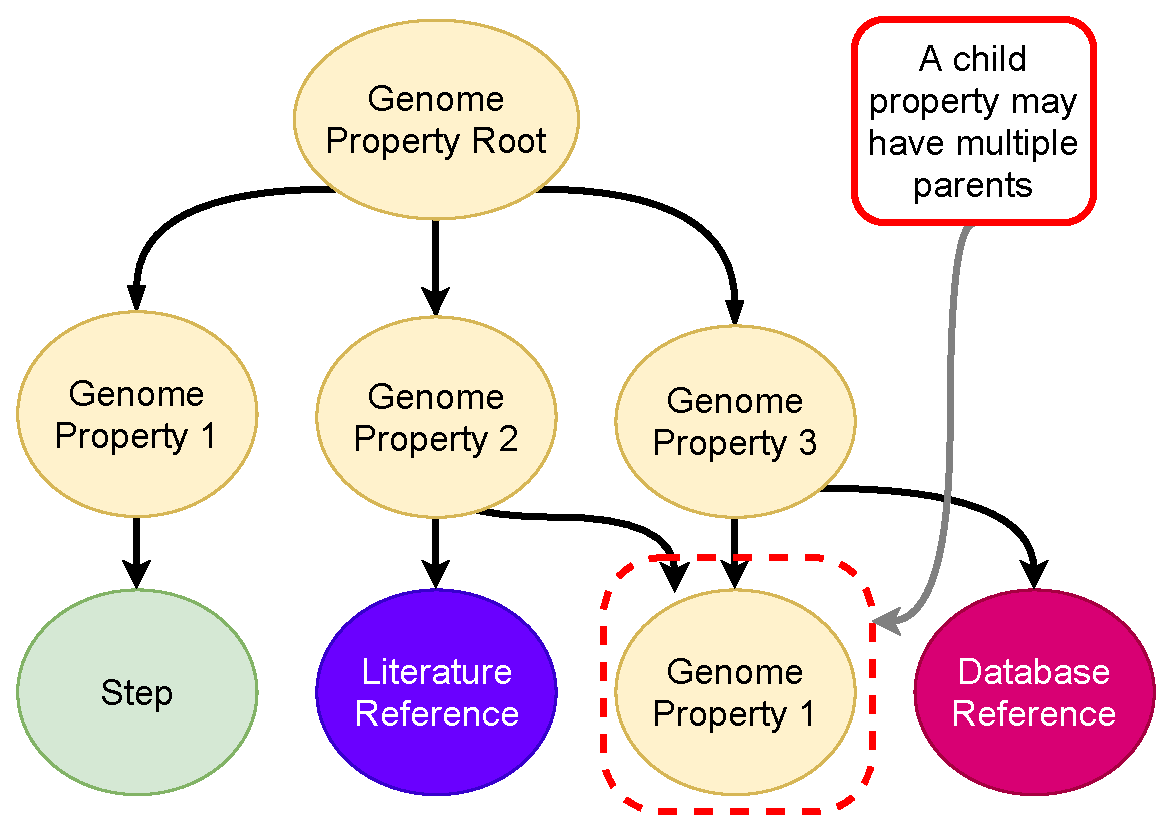
\includegraphics[width=0.90\textwidth]{media/Figure_1A.eps}
	 \caption{Some property objects are the children of others. Database reference, literature reference and step objects are children of property objects. Figure is from \cite{bergstrand2019pygenprop}.}
	 \label{fig:propertytree}
\end{figure}

\begin{figure}[!ht]
  \centering
	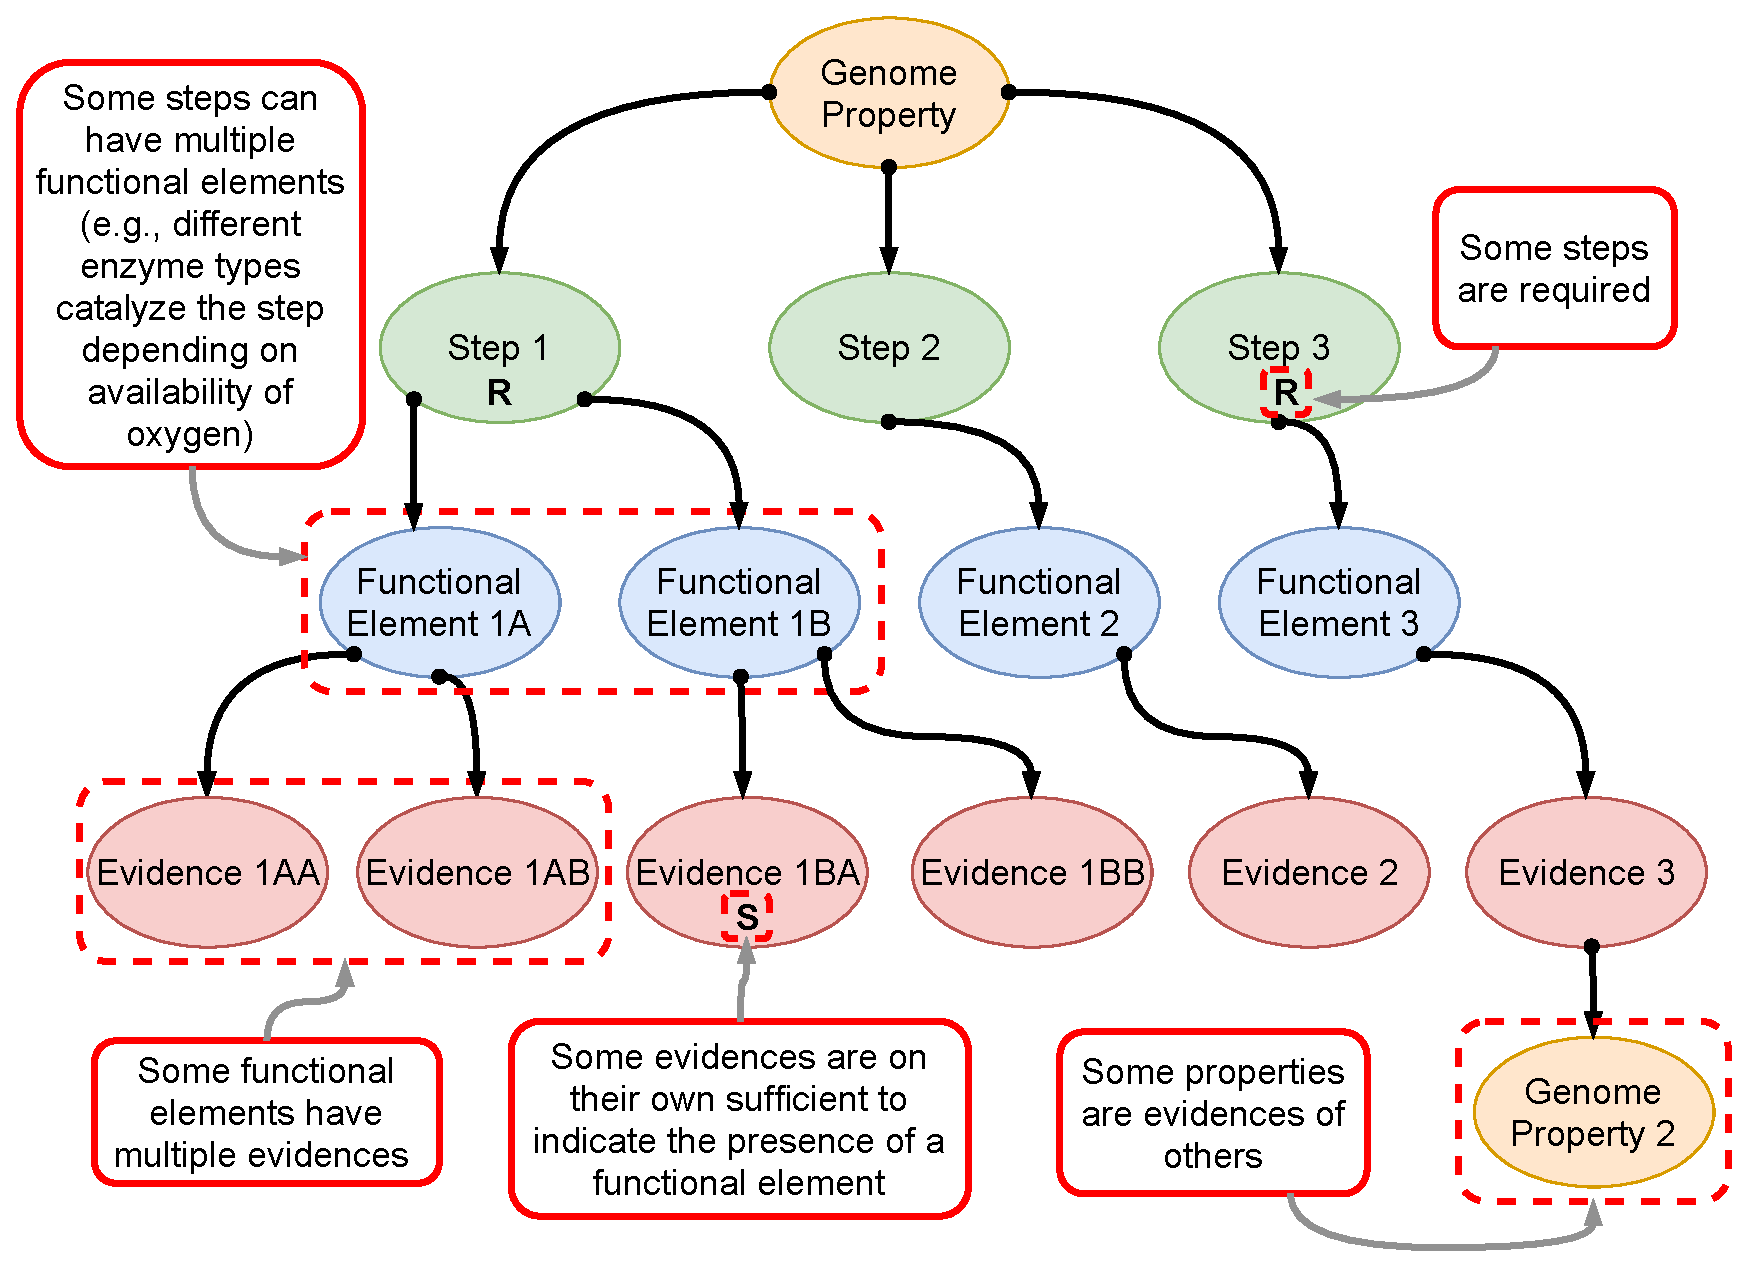
\includegraphics[width=0.90\textwidth]{media/Figure_1B.eps}
	 \caption{Each property is supported by step, functional element, and evidence objects. Figure is from \cite{bergstrand2019pygenprop}.}
	 \label{fig:property}
\end{figure}

\subsection{The Genome Property Class}

The genome property class creates a blueprint for objects which represent individual genome properties. Instantiated objects possess methods, properties (attributes whose return value is generated by a function), and attributes which represents data about the property contained in the property \textbf{DESC} file. Information about property steps, database references and literature references have been abstracted into their own classes. A summary of the methods, properties and attributes of genome property objects can be seem in Table \ref{tab:genome-property-object} and example code below.

\begin{longtable}{|p{2.7cm}|p{2cm}|p{10cm}|}
\caption{A list of methods, properties and attributes of genome property objects.}
\label{tab:genome-property-object}\\
\hline
\textbf{Name} & \textbf{Type} & \textbf{Description} \\ \hline
\endfirsthead
%
\multicolumn{3}{}%
{{\bfseries Table \thetable\ continued from previous page}} \\
\hline
\textbf{Name} & \textbf{Type} & \textbf{Description} \\ \hline
\endhead
%
required\_steps & Property & Return a list of step objects representing steps which are required to support the existence of the property \\ \hline
child\_genome \_property \_identifiers & Property & Return a list of the genome property identifiers of child genome properties which are used as step evidences for the property \\ \hline
to\_json & Method & Serialize the property to a JSON string \\ \hline
databases & Attribute & A list of database objects representing external database references to the property \\ \hline
references & Attribute & A list of literature reference objects representing external articles discussing the property \\ \hline
private\_notes & Attribute & Private internal notes about the property \\ \hline
tree & Attribute & The genome property tree for to which the property belongs \\ \hline
description & Attribute & A complete description for the property \\ \hline
threshold & Attribute & The minimum number of required steps for to which must be assigned YES in order for the property to be assigned PARTIAL rather than NO support during property assignment \\ \hline
type & Attribute & The type of property (e.g. GUILD, CATEGORY, PATHWAY, etc.) \\ \hline
steps & Attribute & A list of step objects representing all steps that can support the existence of the property (including non-required) \\ \hline
public & Attribute & True if the property is publicly released \\ \hline
children & Attribute & A list of child genome property objects representing properties the are used as step evidences by the property \\ \hline
name & Attribute & The name of the property \\ \hline
id & Attribute & The genome property identifier (e.g. GenPropXXXX) \\ \hline
parents & Attribute & A list of parent genome properties objects representing properties that use the property as step evidences \\ \hline
\end{longtable}

\subsubsection{Example code for using genome property objects}

\begin{lstlisting}[language=Python]

property.id
Out: 'GenProp0144'
	
property.name
Out: 'Chlorophyllide a biosynthesis from protoporphyrin IX'

property.parents
Out: List of parent property objects

property.children	
Out: List of child property objects

property.steps
Out: List of step objects		
	
property.databases
Out: List of database reference objects

property.references
Out: List of literature reference objects

\end{lstlisting}

\subsection{The Database Reference Class}

The database reference class allows for the creation of objects which map the property to equivalent records in other databases such as KEGG and Metacyc. They are children of genome property objects. A summary of the methods, properties and attributes of database reference objects can be seem in Table \ref{tab:database-reference-object} and example code below.

\begin{longtable}{|p{2.7cm}|p{2cm}|p{10cm}|}
\caption{A list of methods, properties and attributes of database reference objects.}
\label{tab:database-reference-object}\\
\hline
\textbf{Name} & \textbf{Type} & \textbf{Description}                  \\ \hline
\endfirsthead
%
\multicolumn{3}{c}%
{{\bfseries Table \thetable\ continued from previous page}} \\
\hline
\textbf{Name} & \textbf{Type} & \textbf{Description}                  \\ \hline
\endhead
%
database\_name & Attribute  & The name of the database in questions (e.g. KEGG)           \\ \hline
record\_title & Attribute  & The name of the record in the external database for which the property is equivalent  \\ \hline
record\_ids & Attribute  & The identifier of the record in the external database for which the property is equivalent \\ \hline
\end{longtable}

\subsubsection{Example code for using database reference objects}

\begin{lstlisting}[language=Python]

reference = property.databases[0]
	
reference.database_name
Out: 'MetaCyc'

reference.record_title
Out: 'Pathway: 3,8-divinyl-chlorophyllide a biosynthesis III'

# Returns a list to handle cases where there are multiple identifiers.
reference.record_ids[0] 
Out: 'PWY-7159'

\end{lstlisting}

\subsection{The Literature Reference Class}

The literature reference class lays out the foundation for objects which represent specific articles which support the existence of the property. They are children of genome property objects. A summary of the methods, properties and attributes of literature reference objects can be seem in Table \ref{tab:literature-reference-object} and example code below.

\begin{longtable}{|p{2.7cm}|p{2cm}|p{10cm}|}
\caption{A list of methods, properties and attributes of literature reference objects.}
\label{tab:literature-reference-object}\\
\hline
\textbf{Name} & \textbf{Type} & \textbf{Description}     \\ \hline
\endfirsthead
%
\multicolumn{3}{c}%
{{\bfseries Table \thetable\ continued from previous page}} \\
\hline
\textbf{Name} & \textbf{Type} & \textbf{Description}     \\ \hline
\endhead
%
number  & Attribute  & The number of the reference   \\ \hline
pubmed\_id & Attribute  & The PUBMED identifier of the reference \\ \hline
title   & Attribute  & The title of the literature reference for the property    \\ \hline
authors  & Attribute  & The authors of the literature reference for the property   \\ \hline
citation  & Attribute  & A citation for the literature reference for the property   \\ \hline
\end{longtable}

\subsubsection{Example code for using literature reference objects}

\begin{lstlisting}[language=Python]

reference = property.references[0]
	
reference.pubmed_id
Out: '17370354'

reference.title
Out: 'Recent advances in chlorophyll biosynthesis.'

reference.citation
Out: 'Photosynth Res. 2006;90(2):173-194.'

\end{lstlisting}

\subsection{The Step Class}

The step class is used to generate objects representing individual genome property steps. They are children of parent genome properties. They also have functional elements as children. A summary of the methods, properties and attributes of step objects can be seem in Table \ref{tab:step-object} and example code below.

\begin{longtable}{|p{2.7cm}|p{2cm}|p{10cm}|}
\caption{A list of methods, properties and attributes of step objects.}
\label{tab:step-object}\\
\hline
\textbf{Name}   & \textbf{Type} & \textbf{Description}                             \\ \hline
\endfirsthead
%
\multicolumn{3}{c}%
{{\bfseries Table \thetable\ continued from previous page}} \\
\hline
\textbf{Name}   & \textbf{Type} & \textbf{Description}                             \\ \hline
\endhead
%
name     & Property  & Return the name of the step                             \\ \hline
required    & Property  & Return true if the step is required for assignment of the parent genome property                \\ \hline
property \_identifiers & Property  & Return a list of genome property identifiers of genome properties which are used as evidence for the step          \\ \hline
interpro \_identifiers & Property  & Return a list of InterPro identifiers which are used as evidence for the step (e.g. IPRXXXX)             \\ \hline
consortium \_identifiers & Property  & Return a list of InterPro consortium member database (e.g. PFAM) signature identifiers which are used as evidence for the step (e.g. PFXXXXX) \\ \hline
genome \_properties  & Property  & Return a list of child genome property objects which are used as evidence for the step              \\ \hline
number     & Attribute  & The number of the step                             \\ \hline
parent     & Attribute  & The parent genome property of the step                         \\ \hline
functional \_elements & Attribute  & A list of functional elements which are used to support the existence a step               \\ \hline
\end{longtable}

\subsubsection{Example code for using step objects}

\begin{lstlisting}[language=Python]

step = property.steps[0]
	
step.number
Out: '1'

step.name
Out: 'Magnesium-chelatase subunit ChlD (EC 6.6.1.1)'

step.required
Out: 'True'

step.interpro_identifiers
Out: 'A list of InterPro identifiers (e.g. IPR011776)'

step.consortium_identifiers 
Out: 'A list of consortium signature identifiers (e.g. TIGR02031)'

step.functional_elements
Out: 'A list of functional element objects'

\end{lstlisting}

\subsection{The FunctionalElement Class}

The FunctionalElement class allows for the instantiation of objects which are placed between step object and evidence objects during parsing. Functional elements are not part of the original genome properties database schema and were added by Pygenprop to take into account for certain steps which can be catalysed by multiple enzyme families. For example, it is common that under anoxic conditions organisms will use a different set of enzymes to catalyze a step in a biochemical pathway due to the lack of oxygen present to support the reaction. This issue of having multiple types of enzymes being able to catalyze a step is an open issue on the Genome Properties database Github (see \href{https://github.com/ebi-pf-team/genome-properties/issues/29}{https://github.com/ebi-pf-team/genome-properties/issues/29}). The addition of functional elements is designed to address this issue. A summary of the methods, properties and attributes of FunctionalElement objects can be seem in Table \ref{tab:element-object} and example code below.

\begin{longtable}{|p{2.7cm}|p{2cm}|p{10cm}|}
\caption{A list of methods, properties and attributes of FunctionalElement objects.}
\label{tab:element-object}\\
\hline
\textbf{Name} & \textbf{Type} & \textbf{Description}                 \\ \hline
\endfirsthead
%
\multicolumn{3}{c}%
{{\bfseries Table \thetable\ continued from previous page}} \\
\hline
\textbf{Name} & \textbf{Type} & \textbf{Description}                 \\ \hline
\endhead
%
parent  & Attribute  & The step object for to which the functional element supports       \\ \hline
evidence  & Attribute  & A list of evidence objects that support the existence of the functional element   \\ \hline
name   & Attribute  & The name of the functional element              \\ \hline
id   & Attribute  & The identifier of the functional element            \\ \hline
required  & Attribute  & True if the functional element is required for assignment of the parent genome property \\ \hline
\end{longtable}

\subsubsection{Example code for using FunctionalElement objects}

\begin{lstlisting}[language=Python]

element = step.functional_elements[0]
	
element.id
Out: 'element.id'

element.name
Out: 'Magnesium-chelatase subunit ChlD (EC 6.6.1.1)'

element.required
Out: 'True'

element.evidence
Out: 'A list of evidence objects'

\end{lstlisting}

\subsection{The Evidence Class}

The evidence class allows for the generations of objects which represent individual pieces of evidence which support the existence of functional elements and in turn genome property steps. Pieces of evidence include the presence of InterPro consortium signatures or support for existence of other genome properties found in an organism's genome. A summary of the methods, properties and attributes of evidence objects can be seem in Table \ref{tab:element-object} and example code below.

\begin{longtable}{|p{2.7cm}|p{2cm}|p{10cm}|}
\caption{A list of methods, properties and attributes of evidence objects.}
\label{tab:evidence-object}\\
\hline
\textbf{Name}   & \textbf{Type} & \textbf{Description}                                \\ \hline
\endfirsthead
%
\multicolumn{3}{c}%
{{\bfseries Table \thetable\ continued from previous page}} \\
\hline
\textbf{Name}   & \textbf{Type} & \textbf{Description}                                \\ \hline
\endhead
%
has\_genome \_property & Property  & Return true if the evidence is supported by the existence a genome property                    \\ \hline
property \_identfiers & Property  & Return a list of genome property identifiers of genome properties which are used by the evidence               \\ \hline
interpro \_identifiers & Property  & Return a list InterPro identifiers of genome properties which are used by this evidence (e.g. IPRXXXX)              \\ \hline
consortium \_identifiers & Property  & Return a list of InterPro consortium member database (e.g. PFAM) signature identifiers of genome properties which are used by this evidence (e.g. PFXXXXX) \\ \hline
genome \_properties  & Property  & Return a list of child genome property objects which are used by this evidence                    \\ \hline
parent     & Attribute  & The parent functional element of this evidence                          \\ \hline
gene\_ontology \_terms & Attribute  & The GO term identifiers associated with the InterPro identifiers which are used by the evidence              \\ \hline
evidence \_identifiers & Attribute  & A list of both InterPro and signature identifiers used by the evidence                    \\ \hline
sufficient    & Attribute  & True if the evidence alone can prove the existence of a functional element                   \\ \hline
\end{longtable}

\subsubsection{Example code for using evidence objects}

\begin{lstlisting}[language=Python]

evidence = element.evidence[0]
	
evidence.has_genome_property
Out: 'false'

evidence.sufficient
Out: 'true'

evidence.interpro_identifiers
Out: 'A list of InterPro identifiers (e.g. IPR011776)'

evidence.consortium_identifiers 
Out: 'A list of consortium signature identifiers (e.g. TIGR02031)'

\end{lstlisting}

\subsection{The Genome Properties Tree Class}

Genome properties tree objects, as instantiated from the genome properties tree class, represent the rooted DAG structure of entire Genome Properties database. even though the Genome Properties database is actually a rooted DAG, the name 'tree' is used for the class and tree terminology is used in the object's methods for end user convenience. A rooted DAG is not a tree as its branches can merge together unlike those of a true tree. Tree objects contains a Python dictionary of genome property objects indexed by their property identifiers. In addition, individual property objects point to each other using their child and parent (Fig. \ref{fig:propertytree} and Table \ref{tab:genome-property-object}). These child-parent relationships between property objects are built the genome properties tree object's instantiation. The genome properties tree class allows users to search for specific genome properties, and find root and leaf properties. A summary of the methods, properties and attributes of tree objects can be seem in Table \ref{tab:tree-object} and example code below.

\begin{longtable}{|p{2.7cm}|p{2cm}|p{10cm}|}
\caption{A list of methods, properties and attributes of tree objects.}
\label{tab:tree-object}\\
\hline
\textbf{Name}        & \textbf{Type} & \textbf{Description}                                                               \\ \hline
\endfirsthead
%
\multicolumn{3}{c}%
{{\bfseries Table \thetable\ continued from previous page}} \\
\hline
\textbf{Name}        & \textbf{Type} & \textbf{Description}                                                               \\ \hline
\endhead
%
build\_genome \_property \_connections  & Method  & Iterate through every genome property which is a child of the tree; set these property's parent and child attributes to point to child and parent property objects which are also children of the tree. This method connects property objects to create a rooted DAG structure. \\ \hline
to\_json         & Method  & Serialize the property tree to a JSON string                                                         \\ \hline
create \_metabolism \_database \_mapping\_file & Method  & Write a CSV file which maps from genome property identifiers to the identifiers of equivelent records found in KEGG and Metacyc                                     \\ \hline
root          & Property  & The genome property who has no parent.                                                           \\ \hline
leafs          & Property  & Return a list of genome property objects whose steps are not supported by other genome properties                                            \\ \hline
genome \_property \_identifiers    & Property  & Return a list of the genome property identifiers (e.g. GenPropXXXX) for all genome properties within the database                                        \\ \hline
interpro \_identifiers      & Property  & Return a list of InterPro identifiers which are used as evidence for all steps (e.g. IPRXXXX) within the database                                        \\ \hline
consortium \_identifiers      & Property  & Return a list of InterPro consortium member database (e.g. PFAM) signature identifiers which are used as evidence for the step (e.g. PFXXXXX) within the database                            \\ \hline
consortium \_identifiers \_dataframe   & Property  & Return the above in the form of a pandas DataFrame                                                        \\ \hline
genome \_properties \_dictionary    & Attribute  & A dictionary of genome property objects representing all genome properties within by the database; dictionary is keyed by genome property identifier                               \\ \hline
\end{longtable}

\pagebreak

\subsubsection{Example code for using genome property tree objects}

\begin{lstlisting}[language=Python]

tree = GenomePropertyTree(*property_object_list)
tree_two = parse_genome_properties_flat_file(properties_file_handle)
	
len(tree) # number of properties in the database
Out: 'false'

tree.root
Out: 'The root genome property object'

tree.leafs
Out: 'A list of leaf genome property objects 
     (those with no child properties)'

for genome_property in tree: # Properties in the tree can be iterated.
	print(genome_property.id)
Out: 'Prints all genome property identifiers'

tree['GenProp1127'] # The tree can be rapidly searched
Out: 'The genome property object representing GenProp1127.'

\end{lstlisting}

\subsection{Performance of Pygenprop's Genome Properties database OOP Implementation}

Pygenprop's representation of the Genome Properties database (Version 2.0), a genome properties tree object and its children, takes only up 11.16 MB of random-access memory. This in contrast to the database's original \textbf{genomeProperties.txt} file which takes up only 1.76 MB on disk. The memory usage difference is due the representation of the database as a series of objects and their associated data structures. However, since 11.16 MB is still takes up little memory on a modern machine, more compact data representations for Genome Properties data were not pursued. The size of the database, and its read-only use case, allows for its storage in main memory rather than in an on-disk database such as SQLite \cite{owens2006definitive} or PostgreSQL \cite{momjian2001postgresql}.

Individual genome property objects can be looked up, by property identifier, from within a genome properties tree object within 277 ns ± 7.91 ns. This speed is due property objects being stored within a Python dictionary. Python dictionaries are implemented a hash tables, allowing for quick look ups \cite{van1995python}.

\section{Assignment of Genome Properties to Organism Genomes}

Information contained within the Genome Properties database can be used to assign YES, NO or PARTIAL support for an organism possessing a genetically-derived property such as a biochemical pathway. These assignments of YES, NO or PARTIAL are based on the the presence of InterPro consortium database signatures (e.g PFAMs, TIGRFAMS, etc.) present in protein domain annotations on an organism's genome. These domain annotations are generated by InterProScan \cite{jones2014interproscan}. Some genome properties, in addition to the above signatures, rely on the previous assignments of support for child genome properties for their own assignment. Pygenprop's code for assigning genome properties is based on that of the Genome Properties Perl library (see https://github.com/ebi-pf-team/genome-properties) that ships along side the Genome Properties database. It replicates the library's assignment functionality. Pygenprop assigns properties support from leaf to root using a recursive algorithm (\ref{fig:propertyassignment}). Assignment starts with step evidences and flows up through functional elements and steps and eventually to individual properties (Fig. \ref{fig:propertyassignment}). The rules used for assigning support at different levels are detailed in the subsections below. For each organism that needs to be to have properties assigned an AssignmentCache object is created. This object contains all data required for property assignment and methods for assigning support for properties using this data. A detailed description of this class is also found in the subsections below.

\begin{figure}[!ht]
  \centering
	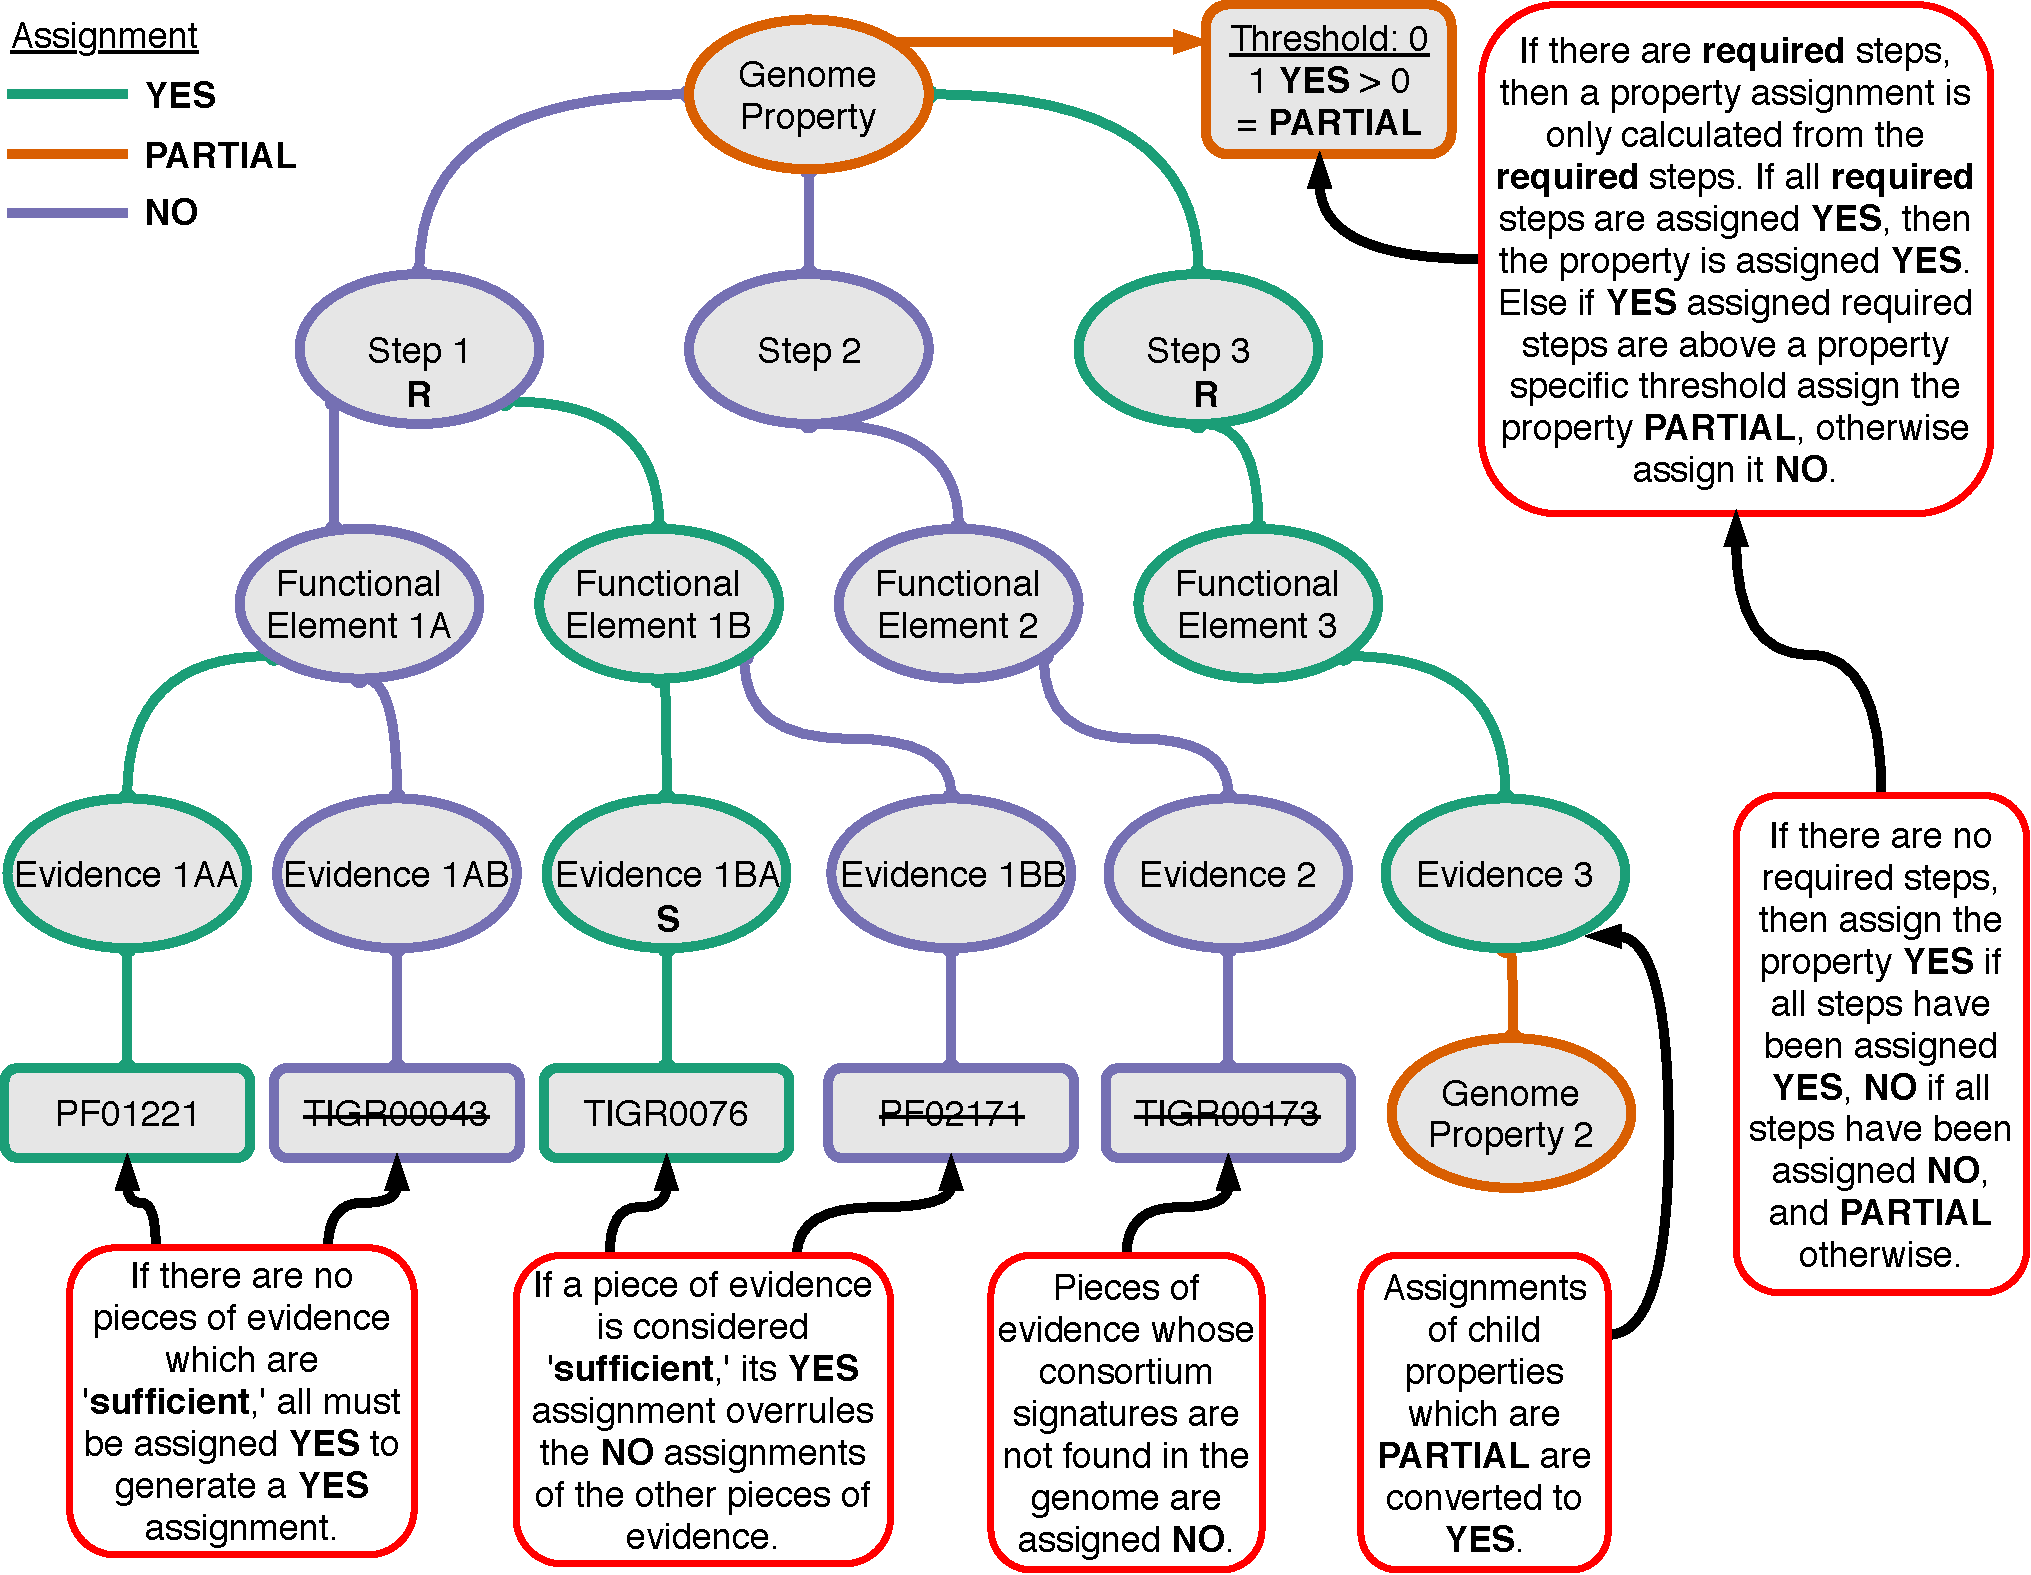
\includegraphics[width=0.90\textwidth]{media/Pygenprop_Assignment.pdf}
	 \caption{An overview of the genome property assignment process used by Pygenprop.}
	 \label{fig:propertyassignment}

\end{figure}

\subsection{The AssignmentCache Class}

AssignmentCache objects, insatiated from the AssignmentCache class, are used to assign genome properties to an organism or metagenome. They can be generated from InterProScan TSV files (protein domain annotation files created by a user), lists of InterPro member database signature identifiers (as could be downloaded from precalculated InterProScan results for UniProt proteomes \cite{uniprot2014uniprot}), or pre-calculated property assignment files previously generated by the Genome Properties Perl library. In the case of InterProScan files, only a deduplicated version of the file's consortium signature identifier column is used. The TSV files are parsed using pandas and pre-calculated property assignment files are parsed using a custom parser. AssignmentCache objects contain two dictionaries for storing previously calculated property and step assignments, respectively. It also contains a Set which is designed to store all InterPro consortium signature identifiers found for an organism's protein domain annotations. The AssignmentCache has a method called \textbf{bootstrap\_assignments} which is use a genome property tree (see Table \ref{tab:tree-object}) object and data stored within itself to calculate all property assignments for an organism. Multiple AssignmentCaches from multiple organisms can be combined together during the creation of GenomePropertiesResultsobjects that allow comparison of properties between organisms. A summary of the methods, properties and attributes of AssignmentCache objects can be seem in Table \ref{tab:tree-object} and example code below.

\begin{longtable}{|p{2.7cm}|p{2cm}|p{10cm}|}
\caption{A list of methods, properties and attributes of AssignmentCache objects.}
\label{tab:assignment-cache-object}\\
\hline
\textbf{Name} & \textbf{Type} & \textbf{Description} \\ \hline
\endfirsthead
%
\multicolumn{3}{c}%
{{\bfseries Table \thetable\ continued from previous page}} \\
\hline
\textbf{Name} & \textbf{Type} & \textbf{Description} \\ \hline
\endhead
%
cache\_property \_assignment & Method & Add a property assignment to the cache \\ \hline
get\_property \_assignment & Method & Return a property assignment from the cache \\ \hline
cache\_step \_assignment & Method & Add a step assignment to the cache \\ \hline
get\_step \_assignment & Method & Retrun a step assignment from the cache \\ \hline
flush\_property \_from\_cache & Method & Remove a property assignment and its associated step assignments from the cache \\ \hline
synchronize \_with\_tree & Method & If a property whose assignment is cached is not found in the tree, remove the assignment and its associated step assignments. This method allows for compatibility between different Genome Properties database versions and pre-calculated assignments. \\ \hline
bootstrap \_assignments & Method & Recursively assign support for properties from leaf to root using an internal set pre-calculated assignments and a InterPro consortium signature identifiers. \\ \hline
bootstrap \_missing\_step \_assignments & Method & Search through a genome property tree to find steps which are not in the cache. Assign these steps NO since they are missing. This method is used when pre-calculated step assignments which result in NO have been omitted to save disk space. \\ \hline
create \_results\_tables & Method & Return two pandas DataFrames representing property and step assignments for the organism \\ \hline
property \_identifiers & Property & Return a list of genome property identifiers (e.g. GenPropXXXX) for properties whose assignment are in the cache \\ \hline
property \_assignments & Attribute & A dictionary of YES, NO and PARTIAL labeled property assignments keyed by genome property identifier. \\ \hline
step \_assignments & Attribute & A doubly nested dictionary of YES, and NO labeled step assignments keyed by genome property identifier and step number. \\ \hline
interpro \_signiture \_accessions & Attribute & A set of InterPro consortium signature identifiers of domains found in the organism's protein domain annotations. \\ \hline
sample\_name & Attribute & The name of the organism or sample. When the AssignmentCache is created from a file, the sample name is set to the filename without file extension. \\ \hline
\end{longtable}

\subsubsection{Example code for using AssignmentCache  objects}

\begin{lstlisting}[language=Python]
tree = parse_genome_properties_flat_file(properties_file_handle)

cache1 = parse_genome_property_longform_file(pre_calculated_file_handle)
cache2 = parse_interproscan_file(interproscan_tsv_file_handle)
cache3 = AssignmentCache(sample_name='E_coli', 
interpro_signature_accessions=identifier_list)

cache2.sample_name
Out: 'C_benthia_SPR155'

cache2.get_property_assignment('GenProp1065')
Out: 'PARTIAL'

cache2.get_step_assignment('GenProp1067', 2) 
Out: 'YES'

# Set GenProp2536 to YES
cache2.cache_property_assignment('GenProp2536', 'YES')

# Set GenProp2539 step two to YES
cache2.cache_step_assignment('GenProp2539', 2, 'YES')

# Remove GenProp2567 from the cache
cache2.flush_property_from_cache('GenProp2567')

# Bootstrap both step and property assignments
cache2.boostrap_assignments(properties_tree=tree)

# Create pandas DataFrames for per organism property
# and step assignments
tables = cache2.create_results_tables(properties_tree=tree)
property_table = tables[0]
step_table = tables[1]

\end{lstlisting}

\subsection{Implemented Assignment Algorithms}

As mentioned above, Pygenprop use recursion, the process of functions calling themselves, to assign YES, NO and PARTIAL support for individual properties found within the genome properties database. During assignment recursion, Pygenprop uses a genome properties tree object to provide it with information about assignment requirements and connections between individual genome properties. In the context of AssignmentCache objects, the support assignment process is referred to as bootstrapping assignments. This is because properties are assigned from a mixture of existing informations such as pre-calculated assignments and InterPro consortium signatures found in an organism's domain annotations. Like in the algorithms used in the Genome Properties Perl library, both properties and steps are given assignments and step assignment are used to assign support for parent properties. It is of note that, during the recursion process, that newly calculated step and property assignments are added to the AssignmentCache object's step and property assignment dictionaries. Successive recursive assignment calculates check these dictionaries first, using the \textbf{get\_property\_assignment} and \textbf{get\_step\_assignment} methods, to find step and property assignment which have already been calculated. Since the Genome Properties database forms a rooted DAG, branches in the parent-child property relationships can merge. Thus there will be property assignments to retrieve from the cache as they have already been calculated in previous recursions. In addition, the step and AssignmentCache dictionaries can be filled with pre-calculated assignments from a file or database. The use of an assignment caching, allows for the assignment process to increase in speed up exponentially as more properties are calculated. Assignments which are already cached are taken as gospel and recursion stops when they are collected from the cache. Recursion also stops when step assignments are calculated for steps which are not supported by the assignment of other genome properties. 

\subsubsection{Assigning support for steps, functional elements and evidences}

Step assignments are calculated recursively from functional element and evidence assignments (Fig. \ref{fig:propertyassignment}). Evidences are assigned YES or NO based on the presence an InterPro consortium signature found in the AssignmentCache's \textbf{interpro \_signiture \_accessions} set (Table \ref{tab:assignment-cache-object}) or a recursively calculated property assignment. The signature identifier or child property to be used specified inside evidence's representative evidence object (Table \ref{tab:evidence-object}) inside the genome property tree object passed to the cache's \textbf{bootstrap\_assignments} function. Evidence are assigned NO if they are not found in the cache's \textbf{interpro \_signiture \_accessions} attribute and YES otherwise. If the evidence is supported by the support assignment of another genome property, then the evidence is only assigned YES if the genome property's assignment is YES or PARTIAL (Fig. \ref{fig:propertyassignment}). Functional elements are assigned YES under two situations: If all underlying evidences have been assigned YES or if a single evidence which sufficient on its own to support the existence of a step is assigned YES (Fig. \ref{fig:propertyassignment}). For example, if As mentioned in Table \ref{tab:evidence-object}, some evidences can be used as the sole piece of evidence for a step. Other than these two situations the functional element is assigned NO. Steps are assigned YES or NO based off the assignments of functional elements (Fig. \ref{fig:propertyassignment}). Steps are assigned YES only if all functional elements of that step have been assigned YES and are assigned NO otherwise. As noted in the above section, assignment results for already calculated steps are checked for before step assignment recursion and are added to the cache after step assignment calculations. If an evidence has a genome property as its child, this property's assignment is calculated creating another recursion cascade.

\subsubsection{Assigning support for non-categorical properties}

Some properties have steps which are required to exist for the property to be assigned YES or PARTIAL. In addition each property is given a \textbf{threshold} attribute (Table \ref{tab:genome-property-object}) which specifies how many required steps must be present before an assignment of PARTIAL support can be applied to the property. If their are required steps for a property, as specified by information contained in a genome property object in the genome property tree, the genome property can only be assigned YES if all required properties are present (Fig. \ref{fig:propertyassignment}). The property is assigned PARTIAL if the number of its required steps assigned YES is greater than its required steps threshold attribute (Fig. \ref{fig:propertyassignment}). If the number of required steps assigned YES is less than or equal to the required steps threshold then the property is assigned NO support. It is important to note that genome property support assignment does note take into account steps which are optional, only those which are required. As noted in the above section, assignment results for already calculated properties are checked for before property assignment recursion and are added to the cache after property assignment calculations. If a property's step's assignment value is not known it is calculated causing a recursion cascade.

\subsubsection{Assigning support for categorical properties}

Categorical properties, such as GenProp0065 Metabolism, do not have any required steps. All steps are optional. Thus a different algorithm is required for their assignment. Categorical properties are only assigned YES if all steps are assigned YES, NO if all steps are assigned NO and PARTIAL otherwise (Fig. \ref{fig:propertyassignment}). Note that the generation of support assignments for categorical properties is unique to Pygenprop and is not performed by the Genome Properties Perl library. The recursion in the Perl library stops before it reaches categorical properties.

\subsection{AssignmentCache and Assignment Algorithm Performance}

For a 2.93 MB InterProScan TSV file containing domain annotations for 4100 \textit{Escherichia\ coli }K12 proteins, the resulting AssignmentCache object was found to be 1.16 MB of main memory before bootstrapping assignments and 1.71 MB after. Assignment bootstrapping was found to take 76.7 ± 15.41 ms for K12 (using a Macbook Pro 13-inch, Late 2013 with an Intel Intel Core i5 2.4 GHz processor). Thus, Pygenprop could calculate property assignments for thousands genomes in only a few minutes. This speed was found to be sufficient. However, further performance gains could be made in the future if assignments were stored inside pandas DataFrames \cite{mckinney2010data} similar to those created by an AssignmentCache object's \textbf{create\_results\_tables} method (Table \ref{tab:assignment-cache-object}), rather than a Python dictionary.

\section{Development of a Framework for Comparing Genome Property Assignments Across Multiple Organisms}

One of the main goals of Pygenprop was to facilitate comparison of the presence/absence of biochemical pathways across organism. In addition, Pygenprop is designed to support making these comparisons programmatically. Specifically, it is designed to provide methods to filter out properties which are shared between organisms to highlight differences in metabolic or functional capabilities across organisms. Having programmatic access to these difference and having them in computationally accessible form will allow future researchers to automate many aspects of pathway analysis, such as complex phenotype prediction and prediction of niche partitioning in the case of microbial ecology contexts.

\subsection{The GenomePropertiesResults Class}

To support programmatic exploration of genome properties assignments Pygenprop includes the GenomePropertiesResults class. Objects of this class takes a series of AssignmentCache objects (Table \ref{tab:assignment-cache-object}), potentially from disparate sources, as input during their instantiation (Fig. \ref{fig:resultscreation}). The per-sample assignments found within these caches are then combined into a multiple sample form. Specifically, they are stored in two indexed pandas DataFrames \cite{mckinney2010data}: One for property level assignments and another for step level assignments (Fig. \ref{fig:resultswithmatchescreation}). Within these DataFrames, assignments are stored in compact NumPy arrays \cite{van2011numpy}. In addition, to these two DataFrames the GenomePropertiesResults class contains a series of functions for filtering down step and property assignments. A summary of the methods, properties and attributes of GenomePropertiesResults objects can be seem in Table \ref{tab:results-object} and example code below.

\begin{figure}[!ht]
  \centering
	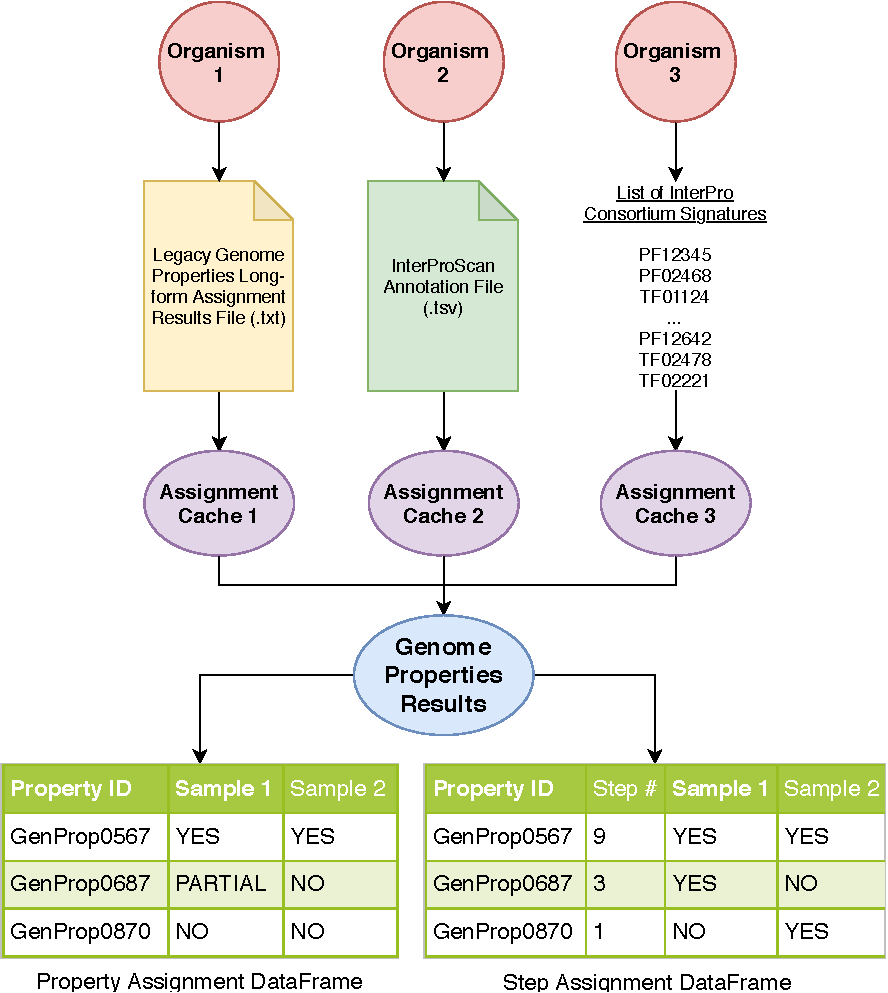
\includegraphics[width=0.85\textwidth]{media/assignment_results_overview.pdf}
	 \caption{GenomePropertiesResults objects are created by combining the AssignmentCache objects generate for multiple organisms. These caches can be generated from disparate sources such as InterProScan results files or lists of InterPro signatures provided by an remote server.}
	 \label{fig:resultscreation}
\end{figure}

\begin{longtable}{|p{2.7cm}|p{2cm}|p{10cm}|}
\caption{A list of methods, properties and attributes of GenomePropertiesResults objects.}
\label{tab:results-object}\\
\hline
\textbf{Name} & \textbf{Type} & \textbf{Description} \\ \hline
\endfirsthead
%
\endhead
%
get\_results & Method & Return the assignment results as a pandas DataFrame for a series of genome properties at either a step or property level \\ \hline
get\_results \_summary & Method & Return a summary of assignment results as a pandas DataFrame for a series of genome properties a either a step or property level \\ \hline
get\_property \_results & Method & Return a list of assignments of support for all samples for a given property \\ \hline
get\_step\_results & Method & Return a list of assignments for all samples for a given property step \\ \hline
to\_json & Method & Serialize the results object as a JSON property tree with results for each sample annotating each property node \\ \hline
to\_assignment \_database & Method & Serialize the results object to a SQLite database file (.micro) \\ \hline
sample\_names & Property & Return the names of all samples used in the creation of the results object. \\ \hline
differing \_property \_results & Property & Return a pandas DataFrame of property assignments with properties whose assignments are the same across all samples filtered out \\ \hline
differing\_step \_results & Property & Return a pandas DataFrame of step assignments with steps whose assignments are the same across all samples filtered out \\ \hline
supported \_property \_results & Property & Return a pandas DataFrame of property assignments with properties whose assignments are NO across all samples filtered out \\ \hline
supported\_step \_results & Property & Return a pandas DataFrame of step assignments with steps whose assignments are NO across all samples filtered out \\ \hline
property\_results & Attribute & A pandas DataFrame of property assignments across all samples \\ \hline
step\_results & Attribute & A pandas DataFrame of step assignments across all samples \\ \hline
tree & Attribute & The genome properties tree object used during instantiation of the results object \\ \hline
\end{longtable}

\subsubsection{Example code for using GenomePropertiesResults objects}

\begin{lstlisting}[language=Python]
tree = parse_genome_properties_flat_file(properties_file_handle)

cache_one = parse_interproscan_file(ipr_file_handle_one)
cache_two = parse_interproscan_file(ipr_file_handle_two)
results = GenomePropertiesResults(cache_one, cache_two, 
                                  properties_tree=property_tree)

results.sample_names
Out: ['E_coli_K12', 'C_luteolum_DSM_273']

results.get_property_result('GenProp1065')
Out: ['NO', 'NO']

results.get_step_result('GenProp1067', 2) 
Out: ['YES', 'NO']

# Get step assignments for GenProp1065 and GenProp1067 with 
# property and step names.
results.get_results('GenProp1065', 'GenProp1067', 
                      steps=True, names=True)
Out:
\end{lstlisting}

\begin{table}[!ht]
\centering
\resizebox{\textwidth}{!}{%
\begin{tabular}{|l|l|l|l|l|l|}
\hline
\textbf{Property\_Identifier} & \textbf{Property\_Name} & \textbf{Step\_Number} & \textbf{Step\_Name} & \textbf{E\_coli\_K12} & \textbf{C\_luteolum\_DSM\_273} \\ \hline
GenProp1065 & Radical SAM/SPASM TIGR04347/TIGR04031 system & 1 & RSAM-partnered protein, Htur\_1727 family & NO & NO \\ \hline
GenProp1065 & Radical SAM/SPASM TIGR04347/TIGR04031 system & 2 & Pseudo-rSAM protein/SPASM domain protein & NO & NO \\ \hline
GenProp1067 & Defense systems & 1 & CRISPR systems & YES & YES \\ \hline
GenProp1067 & Defense systems & 2 & Restriction enzyme system, type I & YES & NO \\ \hline
GenProp1067 & Defense systems & 3 & DNA sulfur modification system dnd & NO & NO \\ \hline
GenProp1067 & Defense systems & 4 & Abortive infection proteins & NO & NO \\ \hline
GenProp1067 & Defense systems & 5 & Complement activation, common pathway 1 & NO & NO \\ \hline
\end{tabular}%
}
\end{table}

\begin{lstlisting}[language=Python]
# Get property assignments for GenProp1065 and GenProp1067
results.get_results('GenProp1065', 'GenProp1067', 
                    steps=False, names=False)
Out:
\end{lstlisting}

\begin{table}[!ht]
\centering
\begin{tabular}{|l|l|l|}
\hline
\textbf{Property\_Identifier} & \textbf{E\_coli\_K12} & \textbf{C\_luteolum\_DSM\_273} \\ \hline
GenProp1065 & NO & NO \\ \hline
GenProp1067 & PARTIAL & PARTIAL \\ \hline
\end{tabular}
\end{table}

\begin{lstlisting}[language=Python]
# Get counts of YES and NO assignments for steps GenProp1065 
# and GenProp1067
results.get_results_summary('GenProp1065', 'GenProp1067', steps=True)
Out:
\end{lstlisting}

\begin{table}[!ht]
\centering
\begin{tabular}{|l|l|l|}
\hline
\textbf{Assignment} & \textbf{E\_coli\_K12} & \textbf{C\_luteolum\_DSM\_273} \\ \hline
NO & 5 & 6 \\ \hline
YES & 2 & 1 \\ \hline
\end{tabular}
\end{table}

\begin{lstlisting}[language=Python]
# Get percentages of YES and NO assignments for steps GenProp1065 
# and GenProp1067
results.get_results_summary('GenProp1065', 'GenProp1067', 
                             steps=True, normalize=True)
Out:
\end{lstlisting}

\begin{table}[!ht]
\centering
\begin{tabular}{|l|l|l|}
\hline
\textbf{Assignment} & \textbf{E\_coli\_K12} & \textbf{C\_luteolum\_DSM\_273} \\ \hline
NO & 71.428571 & 85.714286 \\ \hline
YES & 28.571429 & 14.285714 \\ \hline
\end{tabular}
\end{table}

\subsection{The use of Pandas for Compatibility With the Python Data Science and Machine Learning Software Stack}

Pandas is a Python library for cleaning, filtering and reshaping data. It presents data to users as a DataFrame, in other words a two dimentional data matrix with both column and row names. Pandas dataframe's allow user's to index columns, supporting the rapid joining of datasets. During data analysis it is common to join DataFrames together creating joint datasets. Pandas DataFrames were designed to provide Python with similar functionality to the builtin dataframes presented by other data analysis languages such as R \cite{rprogman}. Both pandas DataFrame objects contained within an GenomePropertiesResults object are built on top of NumPy arrays \cite{mckinney2010data}. NumPy arrays are a compact memory format designed to support vectorized mathematical calculations on both numeric and string data \cite{van2011numpy}. They are roughly equivalent to R vectors \cite{rprogman}. NumPy arrays are used extensively across the entire Python data science stack . This software stack is called SciPy \cite{scipystack}.

Pygenprop presents property and step assignments as pandas DataFrames inside of an GenomePropertiesResults object. These DataFrames allows users to easily query and filter assignments using pandas idioms, and join these assignments to pre-existing metadata. For example, gene expression data (microarray or transcriptomic), culture optimal growth conditions or even host environmental conditions. Once these datasets are joined they can be co-visualized, using libraries such as Bokeh \cite{bokeh} and Seaborn \cite{seaborn}, to help with pattern discovery. Bokeh can even be used to generate data visualization dashboards (small websites which present pre-built charts) that other researchers can use \cite{bokeh}. These dashboards are equivalant to R's Shiny apps. These joined datasets provide great potential as a source of data for data mining or as training sets for machine learning algorithms. Specifically the NumPy arrays inside pandas DataFrames can easily be transferred to machine learning libraries in the SciPy ecosystem such as Scikit-learn \cite{pedregosa2011scikit}, PyTourch \cite{Paszke2017} and Tensorflow \cite{abadi2016tensorflow}. Scikit-learn can be used to cluster the above joint data to mine for patterns of interest as well as build machine learning classifiers which can make predictions based on genome properties assignments. Examples of classifier provided by Scikit-learn include Support Vector Machine (SVM) and Random Forests classifiers \cite{pedregosa2011scikit}.

\subsection{GenomePropertiesResults Performance}

When generated from two assignment caches containing assignments for to bacteria with 4100 and 1877 proteins, respectively, the resulting GenomePropertiesResults object took up 14.4 MB of main memory. Creating the  object took 177 ms ± 10 ms (using a Macbook Pro 13-inch, Late 2013 with an Intel Intel Core i5 2.4 GHz processor). Thus, Pygenprop could create a GenomePropertiesResults object from thousands of assignment caches in only a few tens of minutes. This speed was found to be sufficient. The memory usage is likely due to the using indexed pandas DataFrames. Pandas DataFrames uses up more memory than raw Python or NumPy arrays since pandas allows for the creation of indexed columns which take up more memory but allow for faster look ups. Pygenprop uses these types of columns. If one needed lower memory usage they could store assignments as raw unindexed NumPy arrays inside the GenomePropertiesResults objects rather than pandas DataFrames. 

\section{Extension of the AssignmentCache and GenomePropertiesResults classes to Include Supporting Match Information}

Motifs are a discrete patterns in a protein's sequence which are often associated with the existence of a protein domain. A protein domain is conserved part of a protein's sequence which carries out a specific function for the protein and are evolutionarily conserved. These domains often generate their own discrete three dimensional structures during protein folding. Domain annotation is the process of predicting the placement and function of domains in protein sequences. During genomic analysis it is a common practice to perform domain annotation on an organism's predicted proteins.

Domain annotations of an organism's proteins are created by finding similarities between motifs in an organism's proteins and previously seen motifs of domains from other proteins found in a protein database. If an organism and database motif are highly similar in sequence they are said to form a match. The quality of this match can be quantified by a variety of metrics such as expected value (E-value) score (how likely is the match given the chance of finding it randomly in one of the organism's other proteins) or alignment length (how much of the motif in the protein aligns with the motif in the database). If it is determined that that a match is of high quality, the motif in the organism's protein can be assigned the same name and function as the original domain that the motif matches to in the database.

One tool for performing domain annotation of an organism's proteins is InterProScan which predicts both the type and placement of domains in an organism's proteins and also provides supporting match information to justify its predictions. This supporting information includes E-value scores for matches and predicted domain start and stop points on the annotated protein. The domain annotations and match information generated by InterProScan are stored in TSV files. InterProScan takes a FASTA file \cite{pearson19905} containing an organism's predicted proteins as input.

As mentioned in previous sections, Genome properties are assigned from InterProScan domain annotations of an organism's proteins. These annotations are provided in the above TSV. Specifically predictions of the existence of domains that can be used, either singly or in consort, to uniquely identify enzymes or protein structures which act as evidence for genome property steps. It may be the case that domains used as genome property step evidence's will be found in more than one protein of an organism and some of these proteins may be false positives which may posses the identifying domain (or a similar domain) but do not carry out the genome property step. To filter out these false positives, researchers often want direct access to the match information, such as E-value scores, held within the InterProScan file so they can use it to further filter matches. Alternatively, users may want access to the entire sequence of proteins containing matches so they can be further analysed. For example, the proteins which are predicted to possess a step evidence domain could be compared phylogenetically to reference proteins which are already known carry out a property step in other organisms. Proteins which cluster closely together on phylogenetic trees are more likely to posses the same function than proteins found to be an out group.

Previously with the Genome Properties Perl library, the information required to perform the above analyses were kept in four separate file types: property information was kept in genomeProperties.txt files, assignment information was kept in per-organism long-form property assignment files, protein sequences were kept in per-organism FASTA files \cite{pearson19905} and domain annotations were kept per-organism InterProScan TSV files. If one wanted to find proteins or match information that supported the existence of a genome property step that was assigned YES they would have to write a script to parse all four of these file types, combine the data contained within each and perform searches on this data. These scripts would be difficult and time consuming to write as they would need much boiler plate code to carry out joining the data before analysis. Since above file types are created per-organism, if one wanted to apply such scripts to multiple organisms then these scripts would have to be able to remember which file, and the data held within, belongs to what organism. This tracking would further complicate script development.

Much of the aforementioned boiler plate code has already been integrated into Micromeda. For example, code for parsing the Genome Properties database and the generation of GenomePropertiesResults objects for comparing the presence/absence of genome properties across organisms. To make it easier for users to access match information for proteins which are annotated to have putative domains which support the existence of genome property steps, Pygenprop contains extend versions of both the AssignmentCache and GenomePropertiesResults classes which contain attributes, properties and methods related to accessing the supporting match information that was orignally contained in InterProScan TSV and FASTA files. These classes are called AssignmentCacheWithMatches and GenomePropertiesResultsWithMatches, respectively.

\subsection{Considerations for retention of match information in AssignmentCacheWithMatches and GenomePropertiesResultsWithMatches objects}

Pygenprop can generate pathway annotation files called Micromeda files (see section XXX). These files not only contain property and step assignments for multiple organisms but also contain information supporting the creation of these assignments such as InterProScan match information and protein sequences. However, both FASTA files and InterProScan TSV files, which Micromeda files are ultimately built from, contain information about proteins and domains, respectively, which do not support the existence of genome property steps. Retention of this information is superfluous to the goal of providing supporting information for genome property steps, and would ultimately bloat the file size of the Micromeda files. Thus, in Micromeda files, only retain domain annotations and protein sequences for genome property steps which are assigned YES. In addition, these files only retain E-value scores for domain annotations, and not other types of match metrics, for similar space savings reasons. Since Micromeda files are essentially serializations of GenomePropertiesResultsWithMatches objects, these objects also only retain match information and protein sequences which support genome property steps which are assigned YES. 

Note that only retaining match information and sequences which support steps which are assigned YES generates a corner case. This corner case can be found when a step is which is supported by more than one evidence and is ultimately assigned NO support and one of the evidences is assigned YES (Fig. \ref{fig:propertyassignment}). In this case, the match information supporting the step evidence assigned YES is dropped from the Micromeda files and AssignmentCacheWithMatches objects since its parent step has been assigned NO. The choice to not retain supporting informations for all evidence assigned YES was made in order to reduce the complexity and memory requirements of Micromeda files and is based on the assumption that researchers would rarely look at evidence level supporting information for genome property steps assigned NO.

\subsection{The AssignmentCacheWithMatches Class}

The AssignmentCacheWithMatches class extends the AssignmentCache class via class inheritance. In addition to the attributes, properties and methods inherited from the AssignmentCache class, it also possesses new attributes, properties and methods related to storing match information, such as E-value scores and protein sequences, which support the existence of genome property steps. This match information is stored in a pandas DataFrame within each instantiated AssignmentCacheWithMatches object. These objects are generated from parsing a FASTA file \cite{pearson19905} of an organism's proteins and an InterProScan TSV of domain annotations of these proteins (Fig. \ref{fig:cachewithmatchescreation}). Parsing begins with the TSV file being opened by pandas and the protein sequence identifier, InterPro consortium signature accession, E-value score columns being extracted (Fig. \ref{fig:cachewithmatchescreation}). Each row of the resulting pandas DataFrame corresponds to a protein domain annotation: the identifier of a protein in the FASTA file, the identifier of a matched InterPro consortium signature found in this protein, and the E-value score of that match. The FASTA file is then parsed using Scikit-bio's FASTA file parser (Fig. \ref{fig:cachewithmatchescreation})\cite{scikitbio}. Scikit-bio is a Python bioinformatics library which uses NumPy arrays to store sequence data. The use of NumPy arrays allows it to have superior performance, in terms of memory usage and sequence string manipulation, to competing bioinformatics libraries such a Biopython \cite{cock2009biopython}. Once parsed by Scikit-bio, the FASTA sequences are converted to a pandas DataFrame consisting of a column of protein identifiers and a column of corresponding protein sequences from the original FASTA file. This sequence DataFrame is then merged with the above domain annotation DataFrame using their protein identifier columns creating a third unified DataFrame that is added to a instantiating AssignmentCacheWithMatches object (Fig. \ref{fig:cachewithmatchescreation}). This parsing process creates one AssignmentCacheWithMatches object per pair of FASTA file and corresponding InterProScan TSV file. Note that these objects contain all matches and proteins sequences found in the TSV file and FASTA file. A summary of the methods, properties and attributes of AssignmentCacheWithMatches objects can be seem in Table \ref{tab:assignmentcachewithmatches}. 

\begin{figure}[!ht]
  \centering
	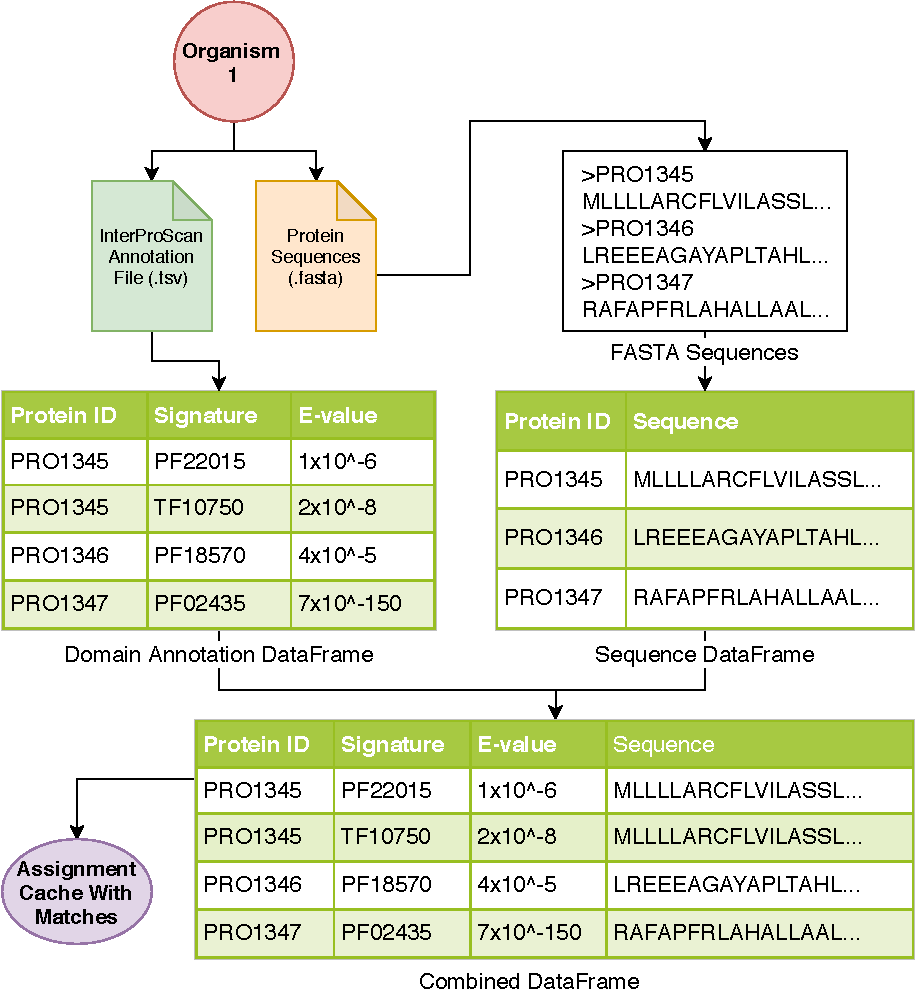
\includegraphics[width=0.70\textwidth]{media/assignmentcachewithmatches_creation.pdf}
	 \caption{AssignmentCacheWithMatches objects are generated from FASTA files of organism proteins and domain annotations of these proteins held in InterProScan TSV files.}
	 \label{fig:cachewithmatchescreation}
\end{figure}

\begin{longtable}{|p{2.7cm}|p{2cm}|p{10cm}|}
\caption{A list of methods, properties and attributes of AssignmentCacheWithMatches objects not possessed by AssignmentCache objects.}
\label{tab:assignmentcachewithmatches}\\
\hline
\textbf{Name} & \textbf{Type} & \textbf{Description}                                                                                    \\ \hline
\endfirsthead
%
\multicolumn{3}{c}%
{{\bfseries Table \thetable\ continued from previous page}} \\
\hline
\textbf{Name} & \textbf{Type} & \textbf{Description}                                                                                    \\ \hline
\endhead
%
matches       & Attribute     & A pandas DataFrame containing domain annotation match information and proteins sequence for an organism \\ \hline
\end{longtable}

\pagebreak

\subsection{The GenomePropertiesResultsWithMatches Class}

\begin{figure}[!ht]
  \centering
	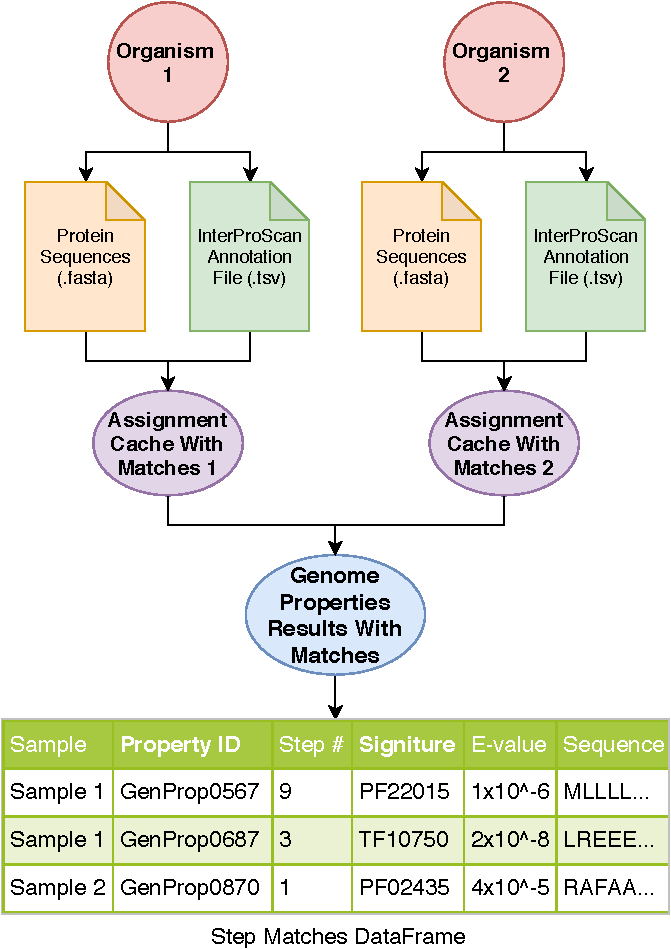
\includegraphics[width=0.60\textwidth]{media/assignment_results_with_matches_overview.pdf}
	 \caption{GenomePropertiesResultsWithMatches objects are created by combining the AssignmentCacheWithMatches objects generate for multiple organisms. These caches are generated from FASTA files of organism proteins and domain annotations of these proteins held in InterProScan TSV files. Property and step assignment DataFrames from  Fig. \ref{fig:resultscreation} are also retained (not shown).}
	 \label{fig:resultswithmatchescreation}
\end{figure}

The GenomePropertiesResultsWithMatches class extends the GenomePropertiesResults class through class class inheritance. In addition to the attributes, properties and methods inherited from the GenomePropertiesResults class, it also possesses new attributes, properties and methods related to storing match information, such as E-value scores and protein sequences, which support the existence of genome property steps in multiple organisms. GenomePropertiesResultsWithMatches objects are generated by combining a series of AssignmentCacheWithMatches objects generated for different organisms (Fig. \ref{fig:resultswithmatchescreation}). Specifically, it combines the \textbf{matches} DataFrame of each input AssignmentCacheWithMatches object into a single DataFrame and indexes this DataFrame by sample name, genome property and step number columns. Having a large combined DataFrame allows for E-value scores and sequences to be compared across organisms. During the creation of this DataFrame, domain matches and proteins sequences which do not support genome property steps are filtered out. The GenomePropertiesResultsWithMatches class provides a variety of convenience functions for accessing match information for proteins which support a step in multiple organisms. It can be also be used to generate FASTA files, using scikit-bio, containing proteins which support the existence of a step in multiple organisms. A summary of the methods, properties and attributes of GenomePropertiesResultsWithMatches objects can be seem in Table \ref{tab:genomepropertyresultswithmatches} and example code below. 

\begin{longtable}{|p{2.7cm}|p{2cm}|p{10cm}|}
\caption{A list of methods, properties and attributes of GenomePropertiesResultsWithMatches objects not possessed by GenomePropertiesResults objects.}
\label{tab:genomepropertyresultswithmatches}\\
\hline
\textbf{Name} & \textbf{Type} & \textbf{Description} \\ \hline
\endfirsthead
%
\multicolumn{3}{c}%
{{\bfseries Table \thetable\ continued from previous page}} \\
\hline
\textbf{Name} & \textbf{Type} & \textbf{Description} \\ \hline
\endhead
%
get\_sample \_matches & Method & Return the step matches DataFrame filtered to include matches from only one sample \\ \hline
get\_property \_matches & Method & Return the step matches DataFrame filtered to include matches from only one genome property \\ \hline
get\_step \_matches & Method & Return the step matches DataFrame filtered to include matches from only one genome property step \\ \hline
get\_supporting \_proteins\_for \_step & Method & Return a list of Scikit-bio sequences objects for proteins which have domain annotations which support a specific property step to a FASTA file \\ \hline
write \_supporting \_proteins\_for \_step\_fasta & Method & Write the protein sequences which have domain annotations which support a specific property step to a FASTA file \\ \hline
top\_step \_matches & Property & Return the matches DataFrame with only the matches with the lowest E-value for each sample and property step retained \\ \hline
step\_matches & Attribute & A pandas DataFrame containing both domain annotations and sequences for proteins which support genome property steps in multiple samples \\ \hline
\end{longtable}

\subsubsection{Example code for using GenomePropertiesResults objects}

\begin{lstlisting}[language=Python]
tree = parse_genome_properties_flat_file(properties_file_handle)

cache_one = parse_interproscan_file_and_fasta_file(ipr_file_one,
                                                   fasta_file_one)
cache_two = parse_interproscan_file_and_fasta_file(ipr_file_two,
                                                   fasta_file_two)
results = GenomePropertiesResultsWithMatches(cache_one, cache_two,          
                                      properties_tree=property_tree)
                                      
results.get_step_matches('GenProp1764', 1)
Out:
\end{lstlisting}

\begin{table}[!ht]
\centering
\resizebox{\textwidth}{!}{%
\begin{tabular}{|l|l|l|l|l|}
\hline
\textbf{Sample\_Name} & \textbf{Signature\_Accession} & \textbf{Protein\_Accession} & \textbf{E-value} & \textbf{Sequence} \\ \hline
C\_chlorochromatii\_CaD3 & PF00994 & NC\_007514.1\_1113 & 7.1e-19 & MITV... \\ \hline
C\_chlorochromatii\_CaD3 & PF00994 & NC\_007514.1\_151 & 1.3e-31 & MRAV… \\ \hline
C\_chlorochromatii\_CaD3 & PF00994 & NC\_007514.1\_1114 & 1.6e-29 & MTFT... \\ \hline
C\_luteolum\_DSM\_273 & PF00994 & NC\_007512.1\_2044 & 2.2e-29 & MPSI... \\ \hline
C\_luteolum\_DSM\_273 & PF00994 & NC\_007512.1\_147 & 1.3e-28 & MAFT... \\ \hline
C\_luteolum\_DSM\_273 & PF00994 & NC\_007512.1\_148 & 3.7e-26 & MLTS... \\ \hline
C\_luteolum\_DSM\_273 & PF01507 & NC\_007512.1\_1607 & 6.1e-38 & MSSA... \\ \hline
C\_luteolum\_DSM\_273 & PF01507 & NC\_007512.1\_1606 & 5.4e-40 & MSRI... \\ \hline
\end{tabular}%
}
\end{table}

\begin{lstlisting}[language=Python]     
# Get only matches for hits with the lowest E-value
# for a single step                                   
results.get_step_matches('GenProp1764', 1, top=True)
Out:
\end{lstlisting}

\begin{table}[!ht]
\centering
\resizebox{\textwidth}{!}{%
\begin{tabular}{|l|l|l|l|l|}
\hline
\textbf{Sample\_Name} & \textbf{Signature\_Accession} & \textbf{Protein\_Accession} & \textbf{E-value} & \textbf{Sequence} \\ \hline
C\_chlorochromatii\_CaD3 & PF00994 & NC\_007514.1\_151 & 1.3e-31 & MRAV… \\ \hline
C\_luteolum\_DSM\_273 & PF01507 & NC\_007512.1\_1606 & 5.4e-40 & MSRI... \\ \hline
\end{tabular}%
}
\end{table}

\pagebreak

\begin{lstlisting}[language=Python]  
# Get only matches for hits with the lowest E-value 
# for a single property for only one sample                                     
results.get_property_matches('GenProp1764', 
                           sample='C_chlorochromatii_CaD3',
                           top=True)
Out:
\end{lstlisting}

\begin{table}[!ht]
\centering
\resizebox{\textwidth}{!}{%
\begin{tabular}{|l|l|l|l|l|}
\hline
\textbf{Step\_Number} & \textbf{Signature\_Accession} & \textbf{Protein\_Accession} & \textbf{E-value} & \textbf{Sequence} \\ \hline
1 & PF00994 & NC\_007514.1\_151 & 1.300000e-31 & MRAE... \\ \hline
2 & PF01687 & NC\_007514.1\_1520 & 3.100000e-33 & MRLI... \\ \hline
\end{tabular}%
}
\end{table}

\subsection{AssignmentCacheWithMatches and GenomePropertiesResultsWithMatches Performance}

For two samples consisting of 1877 and 1774 proteins, respectively, took 80.4 ms ± 1.65 ms and 89.4 ms ± 4.04 ms to parse these samples' FASTA and InterProScan TSVs and generated two AssignmentCacheWithMatches objects. These caches were then combined into a single GenomePropertyResultsWithMatches object in 4.20 s ± 202 ms. Speed tests were performed using a Macbook Pro 13-inch, Late 2013 with an Intel Intel Core i5 2.4 GHz processor. The two assignment caches were found to take 21.26 and 15.31 MB of memory, respectively. The final GenomePropertyResultsWithMatches object was found to take up only 29.8 MB of memory. The size of the objects was determined to be sufficient. A first glance GenomePropertyResultsWithMatches object creation appears to take much time. This time spent is likely due the time taken to join the information found inside each AssignmentCacheWithMatches object. Specifically, the time taken joining pandas DataFrames. At over 4.2 seconds for joining only two caches, scaling analyses to large datasets may become a challenge and opportunities for optimizing this step should be pursued. The GenomePropertyResultsWithMatches object created above was found to be able to be serialized to JSON in 7.08 s ± 1.26 s. This speed was found to be slower than expected and may need to be optimized in the future.

\section{Development of a File Storage Format and Database Interface for Storing Genome Property Assignments and Supporting Match Data}

Once assignments of support are generated for individual genome properties and steps it would be useful to be able to store these assignments for later use or dissemination. With the Genome Properties Perl library, property and step assignments for each organism can be saved to text files written either a custom human readable (see \\ \href{github.com/Micromeda/pygenprop/blob/master/pygenprop/testing/test\_constants/C\_chlorochromatii\_CaD3.txt}{github.com/Micromeda/pygenprop/blob/master/pygenprop/testing/test\_constants/ \\ C\_chlorochromatii\_CaD3.txt}) format or JSON format. Both of these file types are created per-organism and do not contain supporting information such as annotation match scores or proteins sequences. Since these files are created per-organism, a large number of file are required to be tracked or managed if multiple organisms are to be compared. In addition, if users want to retain information about domain annotations and protein sequences which support these assignments, they have to track and manage a series of additional InterProScan TSV and FASTA files for each organism. Tracking, managing and sharing of all these files is  difficult so Pygenprop supports the creation of Micromeda files which combine the information held within these three file types into a single file. This file type can store this information for multiple organisms allowing transfer of entire datasets in a single file between users and computer systems.

\subsection{Selection of a Data Storage Format}

Micromeda's assignment results file format is based off of SQLite3 \cite{owens2006definitive}. During the development several types file types were reviewed before selection of SQLite3 as the preferred format. These formats included, custom text files, binary files, JSON, YAML, and HDF5 files. Custom text or binary files were passed over as they would provide minimal advantage over existing off-the-shelf formats which provide similar performance with little to no development overhead. Javascript Object Notation (JSON) , and Yaml ain't markup language (YAML) \cite{ben2005yaml} were not selected as they are both text encoded files, and, though human readable, take up significantly more space on disk the equivalent binary formats. Hierarchical Data Format 5 (HDF5) \cite{folk2011overview} is a binary format used for storing very large arrays of data. HDF5 lets you define your own data structures inside the the file. It is currently used as the data storage format for Oxford Nanopore sequencers, where it is used to store raw signal information from a sequencing run. The reason for choosing SQLite3 over HDF5 would be the development time required to define Micromeda's own HDF5 data structures (versus SQLite where you have to define these data structures in terms of relational database tables), and SQLite3's compatibility with a broad range of tools and programming languages, and the fact that SQLite3 uses Structured Query Language (SQL) \cite{sql1987guide} for database and access allowing for compatibility with larger server-based database systems such as MySQL \cite{dubois1999mysql} and PostgreSQL \cite{momjian2001postgresql, owens2006definitive}. 

\subsection{The Usage of SQLAlchemy to Provide Expanded Database Connectivity}

Traditional relational databased management systems (DBMS) such as MySQL and PostgreSQL are server processes which continually run on a computer system (i.e. daemons) waiting for input from other programs on the computer or human users \cite{dubois1999mysql, momjian2001postgresql}. They are designed to handle connections from hundreds of programs or users simultaneously, even across computer networks. Users or processes communicate with these DBMS via a domain-specific language (DSL) called SQL \cite{sql1987guide}. SQL is a standard language which can be used to communicate with a verity of database systems. It allows you to define the databases structure, add and remove data, and filter data \cite{sql1987guide}. In contrast to traditional databases, SQLite3 does not run as a server process, but in contrast, is a C library and associated file type which takes SQL strings as input and uses it to manipulate a single file \cite{owens2006definitive}. 

Its important to note that the SQL language has been continually updated since the late 1980s \cite{sql1987guide, ISO9075} and different DBMSs and SQLite itself have each implemented different features of the language and have also added features to their own versions of the language which are only compatible with them (for example new types for database columns). As a result, the SQL written for one DBMS may not be compatible with another. SQLAlchemy \cite{bayer2014sqlalchemy} is a tool which acts as a compatibility layer and allows users to write software which can query from and store data in multiple types of relational DBMSs (Fig. \ref{fig:sqlalchemy}). To preventing incompatibly, SQLAlchemy generates SQL code tailored to each type of DBMS it connects to. It can also allow you to define your relational tables as Python objects and access individual record as Python objects (Fig. \ref{fig:sqlalchemy}). These objects are used by SQLAlchemy to issue SQL commands, a process known as object-relational mapping (see \href{https://en.wikipedia.org/wiki/Object-relational\_mapping}){en.wikipedia.org/wiki/Object-relational\_mapping}) \cite{o2008object}. SQLAlchemy allows you to create, update and delete, and query data from an SQL DBMS without writing a single line in the SQL language.

Pygenprop uses SQLAlchemy to write assignment data and supporting match information to SQLIte3 files. In the context of Pygenprop,we call these files Micromeda files. In addition, due to the use of SQLAlchemy and through the changing of a single line of code, Pygenprop can also write assignments and supporting data to larger, daemon-based, high performance databases such as PostgreSQL or MySQL (Fig. \ref{fig:sqlalchemy}). In addition, the use of SQLAlchemy allows users to write to clustered versions of these databases, such as Postgres-XL (see \href{www.postgres-xl.org}{postgres-xl.org}), allowing the storage of property assignments for hundreds of thousands of organisms.

\begin{figure}[!ht]
  \centering
	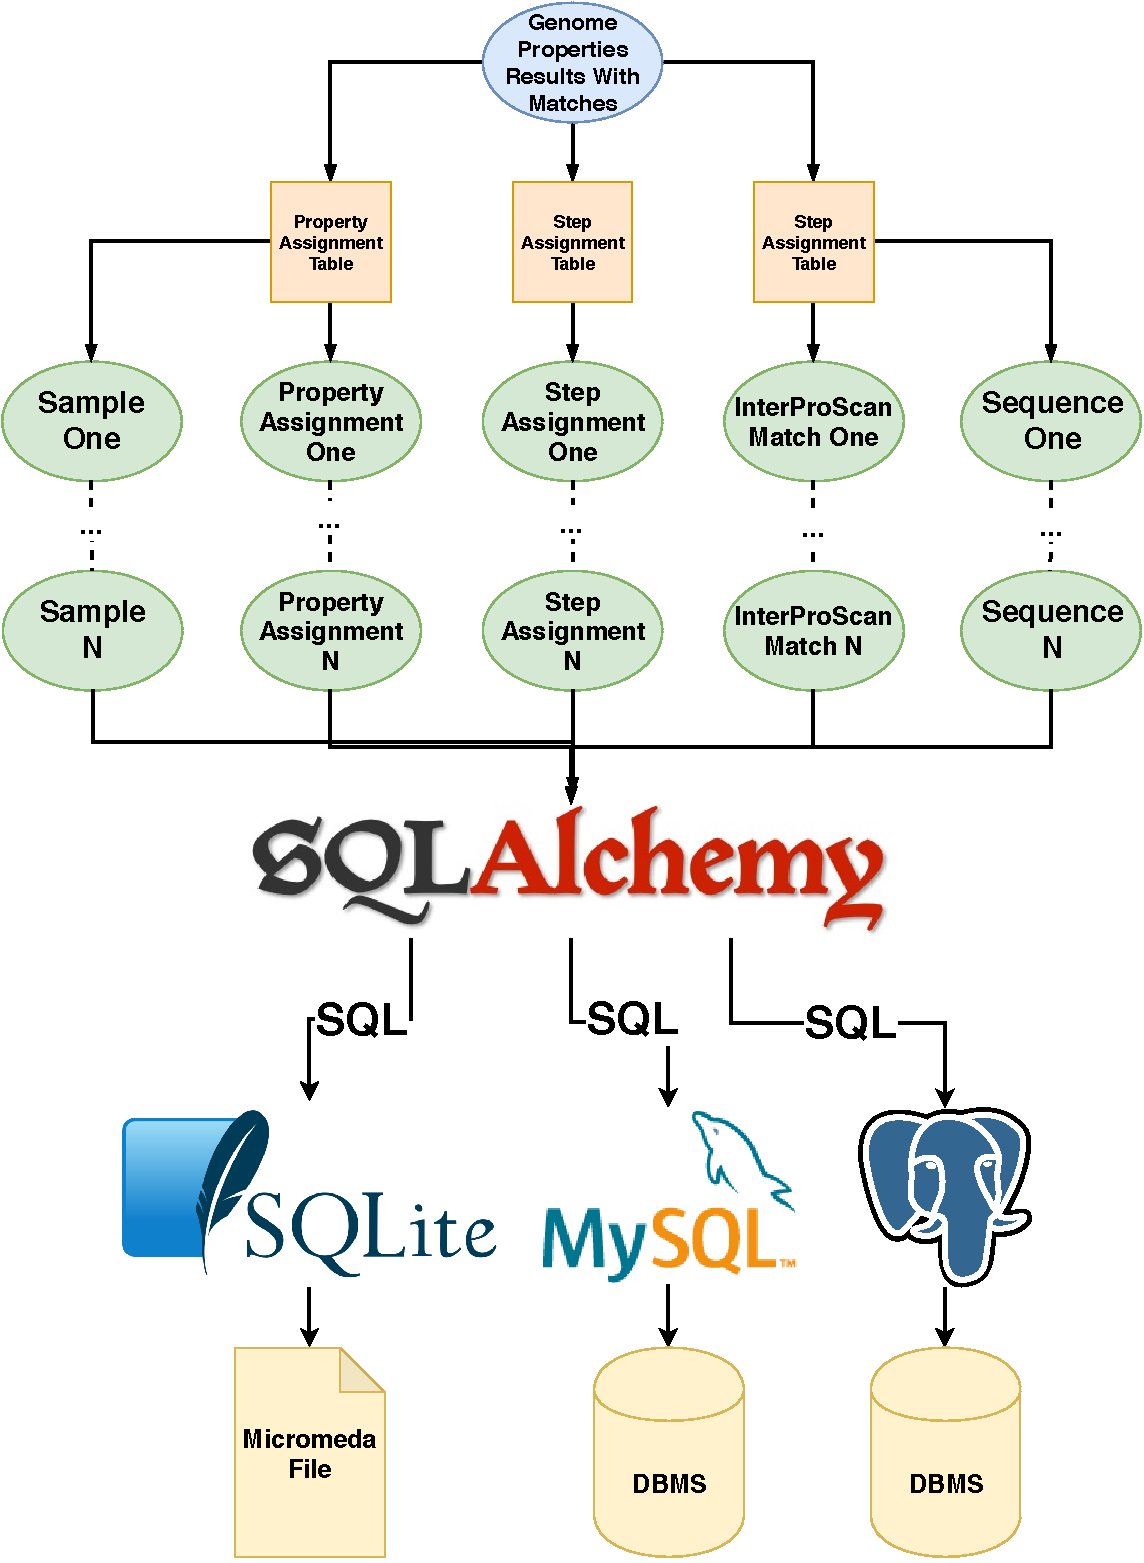
\includegraphics[width=0.65\textwidth]{media/SQLAlchemy.pdf}
	 \caption{SQLAlchemy maps a series of objects generated from an GenomePropertiesResultsWithMatches object to relational database tables.}
	 \label{fig:sqlalchemy}
\end{figure}

\subsection{The Schema of Micromeda File Format}

One of the core goals of Micromeda files is to maintain genome property assignments,  step assignments and associated supporting domain annotations and protein sequences of multiple organisms in a compact a way as possible. This compactness is important as it allows us to keep files sizes, and thus transfer times, to a minimum allowing quick dissemination of datasets. The optimizations which were chosen to support this goal of are listed below:

\begin{itemize}
\item Micromeda files only retain the domain annotation match information and protein sequences for step steps which are assigned YES (as discussed in the section on the GenomePropertiesResultsWithMatches class above).
\item Micromeda files only retain step assignments which are assigned YES. NO assignments are inferred at runtime from properties of a provided GenomePropertiesTree object which are not found in the file.
\item Property and step assignments of support (YES, NO, PARTIAL) are stored as numbers (0, 1, 2) rather than strings in order to save space.
\item The database is fully normalized to the 3rd normal form (3NF) (see \\ \href{en.wikipedia.org/wiki/Database\_normalization}{wikipedia.org/wiki/Database\_normalization}), so that information is only retained once. For example, if a protein sequence supports the existence of multiple property steps of once organism it is only retained once. 
\end{itemize}

Before writing SQLAlchemy classes for relational database tables, SQL schema for Micromeda SQLite3 files was designed visually in the entity-relationship diagramming software called Vertabelo (see \href{www.vertabelo.com}{vertabelo.com}). During the database design the data schema was normalized to the third normal form (3NF). The Micromeda file's final relational table structure can be seen in the schema found in Fig. \ref{fig:micromedaschema}.

\begin{figure}[!ht]
  \centering
	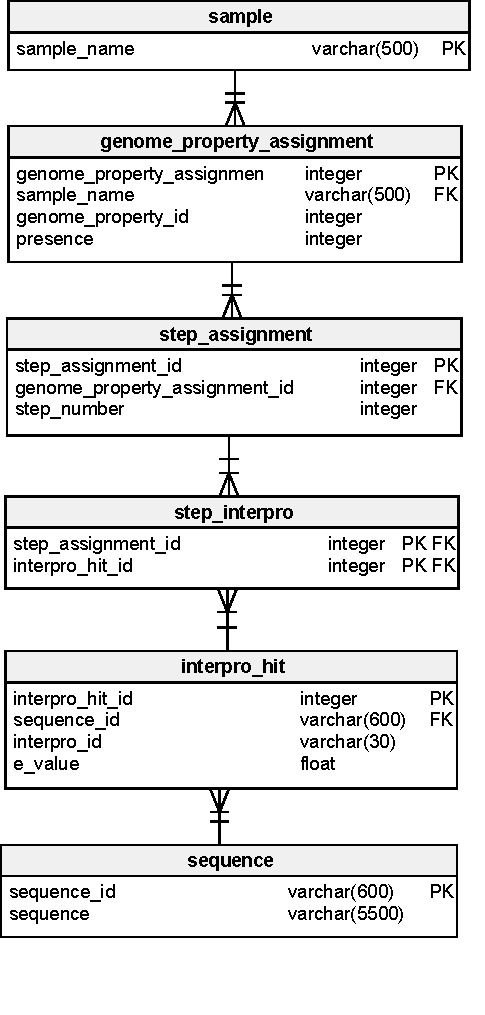
\includegraphics[width=0.50\textwidth]{media/micromeda_schema.pdf}
	 \caption{The SQL schema for Micromeda SQLite3 files contains tables for samples, property assignments, step assignments, a mapping table between step assignments and interpro annotations, interpro annotations and proteins sequences.}
	 \label{fig:micromedaschema}
\end{figure}

\subsection{SQLAlchemy Classes Used By Micromeda}

Pygenprop maintains five SQLAlchemy classes for representing relational tables and records. These objects represent individual property assignments, step assignments, InterProScan domain annotations and protein sequences. They are used to generate SQL statements for both creating SQL tables and queries through SQLAlchemy's object-relational mapping functionality. Attributes, Properties and Methods of these objects are detailed in Tables \ref{tab:sampleobject}, \ref{tab:propertyassignmentobject}, \ref{tab:stepassignmentobject}, \ref{tab:interproscanannotationobject}, \ref{tab:sequenceobject}.

\begin{table}[!ht]
\centering
\caption{A list of methods, properties and attributes of Sample objects.}
\label{tab:sampleobject}
\begin{tabular}{|p{2.7cm}|p{2cm}|p{10cm}|}
\hline
\textbf{Name} & \textbf{Type} & \textbf{Description} \\ \hline
name & Attribute & The name of the sample; for example an organism name \\ \hline
property \_assignments & Attribute & A list of property assignment objects \\ \hline
\end{tabular}
\end{table}

\begin{table}[!ht]
\centering
\caption{A list of methods, properties and attributes of PropertyAssignment objects.}
\label{tab:propertyassignmentobject}
\begin{tabular}{|p{2.7cm}|p{2cm}|p{10cm}|}
\hline
\textbf{Name} & \textbf{Type} & \textbf{Description} \\ \hline
assignment & Property & Return the property's assignment as YES, NO or PARTIAL \\ \hline
identifier & Property & Return the property's identifier (e.g. GenProp0078) \\ \hline
property \_assignment \_identifier & Attribute & A unique numeric identifier for a property assignment of a single sample \\ \hline
property \_number & Attribute & The genome property identifier as a number (e.g. the 0078 of GenProp0078) \\ \hline
numeric \_assignment & Attribute & The property's assignment as the numbers 0, 1, or 2 (equal to YES, NO or PARTIAL) \\ \hline
sample\_name & Attribute & The name of the sample for which the property assignment belongs to \\ \hline
sample & Attribute & The sample object for which the property assignment belongs to \\ \hline
step \_assignments & Attribute & A list of step assignment objects belonging to a single property \\ \hline
\end{tabular}
\end{table}

\begin{table}[!ht]
\centering
\caption{A list of methods, properties and attributes of StepAssignment objects.}
\label{tab:stepassignmentobject}
\begin{tabular}{|p{2.7cm}|p{2cm}|p{10cm}|}
\hline
\textbf{Name} & \textbf{Type} & \textbf{Description} \\ \hline
step \_assignment \_identifier & Attribute & A unique numeric identifier for a step assignment of a single sample \\ \hline
property \_assignment \_identifier & Attribute & The genome property identifier for which the step belongs to as a number (e.g. the 0078 of GenProp0078) \\ \hline
number & Attribute & The step's number \\ \hline
property \_assignment & Attribute & The property assignment object for which the step assignment belongs to \\ \hline
interproscan \_matches & Attribute & A list of interproscan match objects which support the existence of property assignment \\ \hline
\end{tabular}
\end{table}

\begin{table}[!ht]
\centering
\caption{A list of methods, properties and attributes of InterProScanMatch objects.}
\label{tab:interproscanannotationobject}
\begin{tabular}{|p{2.7cm}|p{2cm}|p{10cm}|}
\hline
\textbf{Name} & \textbf{Type} & \textbf{Description} \\ \hline
interproscan \_match \_identifier & Attribute & A unique numeric identifier for an interproscan annotation of a single protein sequence \\ \hline
sequence \_identifier & Attribute & The identifier of a protein sequence \\ \hline
interpro \_signiture & Attribute & The InterPro consortium signature accession of a domain found in a protein sequence \\ \hline
expected\_value & Attribute & The expected value of the match between a motif found in the protein and annotated domain \\ \hline
step \_assignments & Attribute & A list of step assignment objects which are supported by the InterProScan annotation \\ \hline
sequence & Attribute & The sequence object which the InterProScan annotation annotates. \\ \hline
\end{tabular}
\end{table}

\begin{table}[!ht]
\centering
\caption{A list of methods, properties and attributes of Sequence objects.}
\label{tab:sequenceobject}
\begin{tabular}{|p{2.7cm}|p{2cm}|p{10cm}|}
\hline
\textbf{Name} & \textbf{Type} & \textbf{Description} \\ \hline
identifer & Attribute & The identifier of a protein sequence \\ \hline
sequence & Attribute & The protein sequence of the protein \\ \hline
\end{tabular}
\end{table}

\subsection{Writing Micromeda Files}

Both GenomePropertiesResults and GenomePropertiesResultsWithMatches objects provide \textbf{to\_assignment\_database} method. This method takes a SQLAlchemy engine object which can be created to point towards a SQLite3 or larger, process-based relational database. Once called this method converts the the results objects, pandas DataFrames to a series of SQLAlchemy objects detailed above and then use SQLAlchemy to write these objects to the database. Code for writing Micromeda files can be found below.

\begin{lstlisting}[language=Python]  

# A SQLAlchemy engine object can be created
# for a variety of SQL databases
engine = create_engine('sqlite:///data.micro')
results.to_assignment_database(engine)

\end{lstlisting}

\subsection{Reading Micromeda Files}

The reading of assignments from Micromeda files or databases is facilitated by the \textbf{load\\ \_assignment\_caches\_from\_database} and \textbf{load\_assignment\_caches\_from\_database \\ \_with\_matches} functions of Pyegenprop's results module. These functions produce lists of AssignmentCache, or AssignmentCacheWithMatches objects , respectively. These lists are then be combined to form GenomePropertiesResults or GenomePropertiesResultsWithMatches objects. Code for reading Micromeda files can be found below.

\begin{lstlisting}[language=Python]  
tree = parse_genome_properties_flat_file(properties_file_handle)
engine = create_engine('sqlite:///data.micro')

caches = load_assignment_caches_from_database_with_matches(engine)

results = GenomePropertiesResultsWithMatches(*caches,          
                                properties_tree=property_tree)
\end{lstlisting}

\subsection{Micromeda File Performance}

For two samples consisting of 1877 and 1774 proteins a representative GenomePropertiesResultsWithMatches was generated. This object was found to be able to be serialized to a Micromeda file in 29.4 s ± 829 ms. This Micromeda file was found to be approximately one fifth the size of the original files used to create the GenomePropertiesResultsWithMatches objects (Fig. \ref{fig:micromedafilesize}). This Micromeda file was found to be able to be reconstituted back into GenomePropertiesResultsWithMatches object in 6.28 s ± 1.33 s. Though the speed to read Micromeda files was found to be sufficient, writing performance was found to be poor and should be further optimized. Currently, records for individual assignments, annotations and sequences are inserted one at a time into the micromeda file. Matching these inserts together before writing could further improve Micromeda file writing performance.

\begin{figure}[!ht]
  \centering
	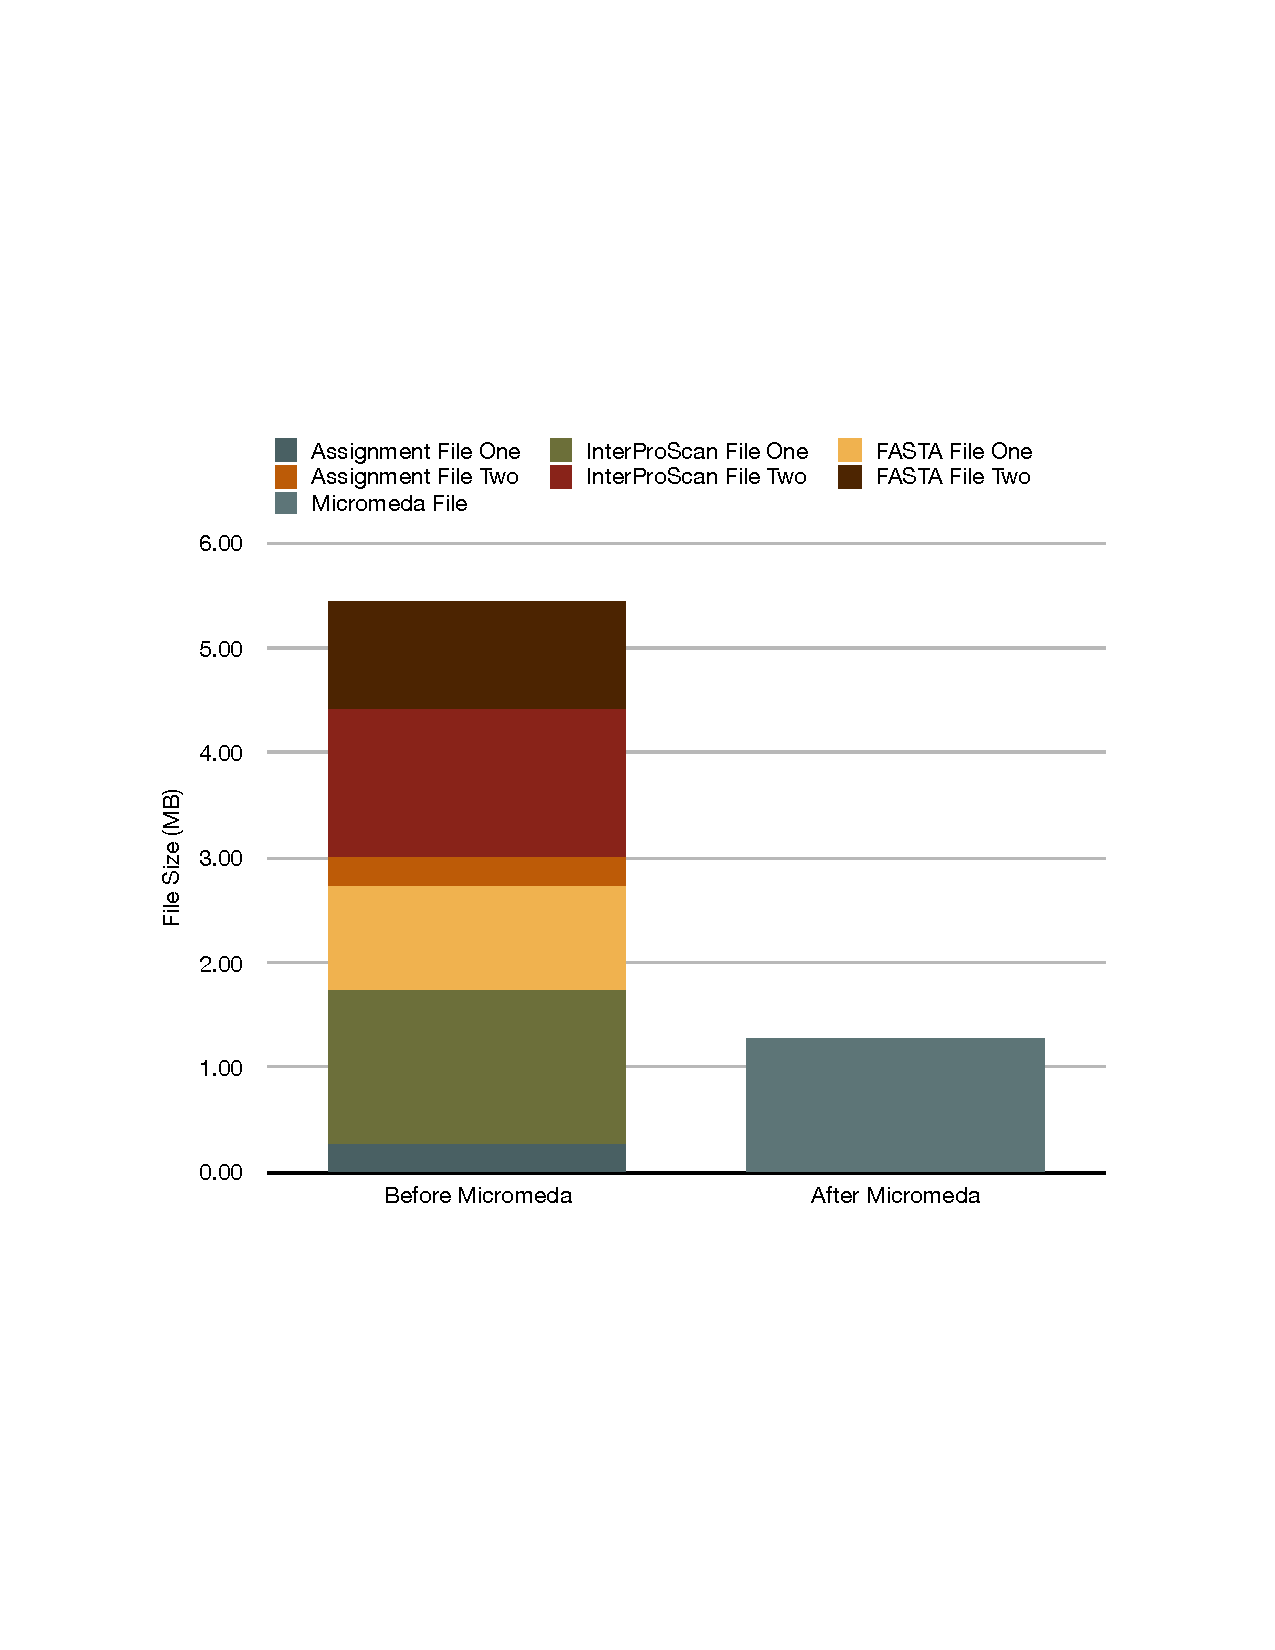
\includegraphics[width=0.80\textwidth]{media/micromeda_file_size.pdf}
	 \caption{Pathway analysis for two samples originally required the tracking of at least three types of files per organism. With Micromeda the information contained within these files is combined and reduced, allowing property assignment relevant information to be stored on one filth the disk space.}
	 \label{fig:micromedafilesize}
\end{figure}

\section{Development of an In-Memory Transfer Format for Property Assignments and Supporting Match Information}

When writing software for pathway analysis it may be of interest to be able to rapidly transfer datasets between machines via memory-to-memory transfer. For example the transfer of datasets between machines which are part of a same high performance computing cluster. Pygenprop is capable of serializing GenomePropertyResultsWithMatches objects into at format optimized for this use case. In the use case of a format memory-to-memory transfer between machines the key performance metric is the serialization/deserialization speed of GenomePropertyResultsWithMatches to the format and the Message Pack (msgpack) format was selected to support this goal.

\subsection{The Selection of Msgpack}

Several formats were reviewed to support the network transfer of assignment and supporting match information transfer between machines. These included: JSON, Google Protocol Buffers (ProtoBuffs), and msgpack. JSON has been the gold standard for transferring information between computer systems for over a decade. However, JSON it is text format and in the past three years several binary alternatives such as ProtoBuffs and Msgpack have emerged that can store the same amount data in less space, allowing for faster transfers. In addition, these formats provide faster serialization/deserialization speed. JSON was rejected due to its spoor serialization/deserialization speed. Msgpack was selected over ProtoBuffs as it had higher compatibility with pandas. Specially, pandas provides methods, though experimental, for serializing DataFrames to msgpack.

\subsection{Serialization and Deserialization of GenomePropertyResultsWithMatches to Msgpack}

GenomePropertyResultsWithMatches objects have a method called \textbf{to\_msagpack} which supports serializing these objects to a msgpack binary stream. The serialization process simply involves calling pandas \textbf{to\_msgpack} function on the GenomePropertyResultsWithMatches object's pandas DataFrames. For deserialization, the process is run in reverse, using the function \textbf{load\_results\_from\_msgpack} of Pygenprop's results module, converting the msgpack binary stream to a GenomePropertyResultsWithMatches object. Code for serializing and deserializing GenomePropertyResultsWithMatches objects can be found below.

\subsection{Msgpack Serialization and Deserialization Performance}

For two samples consisting of 1877 and 1774 proteins a representative GenomePropertiesResultsWithMatches was generated. This object was found to be able to be serialized to a msgpack binary in 29.5 ms ± 270 µs and and deserialized in 54 ms ± 922 µs. The msgpack binary was found to take up 4.36 MB of memory. Both the speed of serialization and the memory used by message pack objects was determined to be sufficient. If lower memory usage is required the GenomePropertiesResultsWithMatches object's step matches DataFrame (Table \ref{tab:genomepropertyresultswithmatches}) could be normalized into two DataFrames, one for storing annotation information and another for storing sequencing information. The data in each of these DataFrames, even when added together, would be smaller than the previous step matches DataFrame since values such as sequences will only be stored once.

\section{Verification and Automated Testing}

Pygenprop has extensive end-to-end and unit tests for its codebase. There are currently 104 unit test written to test the functionality of the majority of code functions. These tests cover 94\% of lines in the codebase. End-to-end test for the libraries involves the creation JSON representations of a GenomePropertiesResults object created from the InterProScan results of two organisms. This test can be run using different versions of the Genome Properties database ensuring compatibility over time.

\section{Future Improvements}



\section{Summary}
